%  LaTeX support: latex@mdpi.com 
%  For support, please attach all files needed for compiling as well as the log file, and specify your operating system, LaTeX version, and LaTeX editor.

%=================================================================
\documentclass[software,article,submit,pdftex,moreauthors]{Definitions/mdpi}
\usepackage[dvipsnames]{xcolor}
\usepackage{listings}

\usepackage{xcolor}
\usepackage{listings}
\usepackage{listingstyles}

%\documentclass[preprints,article,submit,pdftex,moreauthors]{Definitions/mdpi} 
% For posting an early version of this manuscript as a preprint, you may use "preprints" as the journal. Changing "submit" to "accept" before posting will remove line numbers.

% Below journals will use APA reference format:
% admsci, behavsci, businesses, econometrics, economies, education, ejihpe, famsci, games, humans, ijcs, ijfs, journalmedia, jrfm, languages, psycholint, publications, tourismhosp, youth

% Below journals will use Chicago reference format:
% arts, genealogy, histories, humanities, jintelligence, laws, literature, religions, risks, socsci

%--------------------
% Class Options:
%--------------------
%----------
% journal
%----------
% Choose between the following MDPI journals:
% accountaudit, acoustics, actuators, addictions, adhesives, admsci, adolescents, aerobiology, aerospace, agriculture, agriengineering, agrochemicals, agronomy, ai, air, algorithms, allergies, alloys, amh, analytica, analytics, anatomia, anesthres, animals, antibiotics, antibodies, antioxidants, applbiosci, appliedchem, appliedmath, appliedphys, applmech, applmicrobiol, applnano, applsci, aquacj, architecture, arm, arthropoda, arts, asc, asi, astronomy, atmosphere, atoms, audiolres, automation, axioms, bacteria, batteries, bdcc, behavsci, beverages, biochem, bioengineering, biologics, biology, biomass, biomechanics, biomed, biomedicines, biomedinformatics, biomimetics, biomolecules, biophysica, biosensors, biosphere, biotech, birds, blockchains, bloods, blsf, brainsci, breath, buildings, businesses, cancers, carbon, cardiogenetics, catalysts, cells, ceramics, challenges, chemengineering, chemistry, chemosensors, chemproc, children, chips, cimb, civileng, cleantechnol, climate, clinbioenerg, clinpract, clockssleep, cmd, cmtr, coasts, coatings, colloids, colorants, commodities, complications, compounds, computation, computers, condensedmatter, conservation, constrmater, cosmetics, covid, crops, cryo, cryptography, crystals, csmf, ctn, curroncol, cyber, dairy, data, ddc, dentistry, dermato, dermatopathology, designs, devices, diabetology, diagnostics, dietetics, digital, disabilities, diseases, diversity, dna, drones, dynamics, earth, ebj, ecm, ecologies, econometrics, economies, education, eesp, ejihpe, electricity, electrochem, electronicmat, electronics, encyclopedia, endocrines, energies, eng, engproc, ent, entomology, entropy, environments, epidemiologia, epigenomes, esa, est, famsci, fermentation, fibers, fintech, fire, fishes, fluids, foods, forecasting, forensicsci, forests, fossstud, foundations, fractalfract, fuels, future, futureinternet, futureparasites, futurepharmacol, futurephys, futuretransp, galaxies, games, gases, gastroent, gastrointestdisord, gastronomy, gels, genealogy, genes, geographies, geohazards, geomatics, geometry, geosciences, geotechnics, geriatrics, glacies, grasses, greenhealth, gucdd, hardware, hazardousmatters, healthcare, hearts, hemato, hematolrep, heritage, higheredu, highthroughput, histories, horticulturae, hospitals, humanities, humans, hydrobiology, hydrogen, hydrology, hygiene, idr, iic, ijerph, ijfs, ijgi, ijmd, ijms, ijns, ijpb, ijt, ijtm, ijtpp, ime, immuno, informatics, information, infrastructures, inorganics, insects, instruments, inventions, iot, j, jal, jcdd, jcm, jcp, jcs, jcto, jdad, jdb, jeta, jfb, jfmk, jimaging, jintelligence, jlpea, jmahp, jmmp, jmms, jmp, jmse, jne, jnt, jof, joitmc, joma, jop, jor, journalmedia, jox, jpbi, jpm, jrfm, jsan, jtaer, jvd, jzbg, kidney, kidneydial, kinasesphosphatases, knowledge, labmed, laboratories, land, languages, laws, life, lights, limnolrev, lipidology, liquids, literature, livers, logics, logistics, lubricants, lymphatics, machines, macromol, magnetism, magnetochemistry, make, marinedrugs, materials, materproc, mathematics, mca, measurements, medicina, medicines, medsci, membranes, merits, metabolites, metals, meteorology, methane, metrics, metrology, micro, microarrays, microbiolres, microelectronics, micromachines, microorganisms, microplastics, microwave, minerals, mining, mmphys, modelling, molbank, molecules, mps, msf, mti, multimedia, muscles, nanoenergyadv, nanomanufacturing, nanomaterials, ncrna, ndt, network, neuroglia, neurolint, neurosci, nitrogen, notspecified, nursrep, nutraceuticals, nutrients, obesities, oceans, ohbm, onco, oncopathology, optics, oral, organics, organoids, osteology, oxygen, parasites, parasitologia, particles, pathogens, pathophysiology, pediatrrep, pets, pharmaceuticals, pharmaceutics, pharmacoepidemiology, pharmacy, philosophies, photochem, photonics, phycology, physchem, physics, physiologia, plants, plasma, platforms, pollutants, polymers, polysaccharides, populations, poultry, powders, preprints, proceedings, processes, prosthesis, proteomes, psf, psych, psychiatryint, psychoactives, psycholint, publications, purification, quantumrep, quaternary, qubs, radiation, reactions, realestate, receptors, recycling, regeneration, religions, remotesensing, reports, reprodmed, resources, rheumato, risks, robotics, rsee, ruminants, safety, sci, scipharm, sclerosis, seeds, sensors, separations, sexes, signals, sinusitis, siuj, skins, smartcities, sna, societies, socsci, software, soilsystems, solar, solids, spectroscj, sports, standards, stats, std, stresses, surfaces, surgeries, suschem, sustainability, symmetry, synbio, systems, tae, targets, taxonomy, technologies, telecom, test, textiles, thalassrep, therapeutics, thermo, timespace, tomography, tourismhosp, toxics, toxins, transplantology, transportation, traumacare, traumas, tropicalmed, universe, urbansci, uro, vaccines, vehicles, venereology, vetsci, vibration, virtualworlds, viruses, vision, waste, water, wem, wevj, wild, wind, women, world, youth, zoonoticdis

%---------
% article
%---------
% The default type of manuscript is "article", but can be replaced by: 
% abstract, addendum, article, benchmark, book, bookreview, briefcommunication, briefreport, casereport, changes, clinicopathologicalchallenge, comment, commentary, communication, conceptpaper, conferenceproceedings, correction, conferencereport, creative, datadescriptor, discussion, entry, expressionofconcern, extendedabstract, editorial, essay, erratum, fieldguide, hypothesis, interestingimages, letter, meetingreport, monograph, newbookreceived, obituary, opinion, proceedingpaper, projectreport, reply, retraction, review, perspective, protocol, shortnote, studyprotocol, supfile, systematicreview, technicalnote, viewpoint, guidelines, registeredreport, tutorial,  giantsinurology, urologyaroundtheworld
% supfile = supplementary materials

%----------
% submit
%----------
% The class option "submit" will be changed to "accept" by the Editorial Office when the paper is accepted. This will only make changes to the frontpage (e.g., the logo of the journal will get visible), the headings, and the copyright information. Also, line numbering will be removed. Journal info and pagination for accepted papers will also be assigned by the Editorial Office.

%------------------
% moreauthors
%------------------
% If there is only one author the class option oneauthor should be used. Otherwise use the class option moreauthors.

%---------
% pdftex
%---------
% The option pdftex is for use with pdfLaTeX. Remove "pdftex" for (1) compiling with LaTeX & dvi2pdf (if eps figures are used) or for (2) compiling with XeLaTeX.

%=================================================================
% MDPI internal commands - do not modify
\firstpage{1} 
\makeatletter 
\setcounter{page}{\@firstpage} 
\makeatother
\pubvolume{1}
\issuenum{1}
\articlenumber{0}
\pubyear{2025}
\copyrightyear{2025}
%\externaleditor{Firstname Lastname} % More than 1 editor, please add `` and '' before the last editor name
\datereceived{ } 
\daterevised{ } % Comment out if no revised date
\dateaccepted{ } 
\datepublished{ } 
%\datecorrected{} % For corrected papers: "Corrected: XXX" date in the original paper.
%\dateretracted{} % For retracted papers: "Retracted: XXX" date in the original paper.
\hreflink{https://doi.org/} % If needed use \linebreak
%\doinum{}
%\pdfoutput=1 % Uncommented for upload to arXiv.org
%\CorrStatement{yes}  % For updates
%\longauthorlist{yes} % For many authors that exceed the left citation part

%=================================================================
% Add packages and commands here. The following packages are loaded in our class file: fontenc, inputenc, calc, indentfirst, fancyhdr, graphicx, epstopdf, lastpage, ifthen, float, amsmath, amssymb, lineno, setspace, enumitem, mathpazo, booktabs, titlesec, etoolbox, tabto, xcolor, colortbl, soul, multirow, microtype, tikz, totcount, changepage, attrib, upgreek, array, tabularx, pbox, ragged2e, tocloft, marginnote, marginfix, enotez, amsthm, natbib, hyperref, cleveref, scrextend, url, geometry, newfloat, caption, draftwatermark, seqsplit
% cleveref: load \crefname definitions after \begin{document}

%=================================================================
% Please use the following mathematics environments: Theorem, Lemma, Corollary, Proposition, Characterization, Property, Problem, Example, ExamplesandDefinitions, Hypothesis, Remark, Definition, Notation, Assumption
%% For proofs, please use the proof environment (the amsthm package is loaded by the MDPI class).

%=================================================================
% Full title of the paper (Capitalized)
\Title{Enabling Progressive Server-Side Rendering for Traditional Web Template Engines with Java Virtual Threads}

% MDPI internal command: Title for citation in the left column
\TitleCitation{Enabling Progressive Server-Side Rendering for Traditional Template Engines with Java Virtual Threads}

% Author Orchid ID: enter ID or remove command
\newcommand{\orcidauthorA}{0009-0009-1863-3782} % Add \orcidA{} behind the author's name
\newcommand{\orcidauthorB}{0000-0002-4281-3195} % Add \orcidB{} behind the author's name

% Authors, for the paper (add full first names)
\Author{Bernardo Pereira $^{1}$\orcidA{}, Fernando Miguel Carvalho $^{1,*}$ \orcidB{}}

%\longauthorlist{yes}

% MDPI internal command: Authors, for metadata in PDF
\AuthorNames{Bernardo Pereira, Miguel Carvalho}

% MDPI internal command: Authors, for citation in the left column, only choose below one of them according to the journal style
% If this is a Chicago style journal 
% (arts, genealogy, histories, humanities, jintelligence, laws, literature, religions, risks, socsci): 
% Lastname, Firstname, Firstname Lastname, and Firstname Lastname.

% If this is a APA style journal 
% (admsci, behavsci, businesses, econometrics, economies, education, ejihpe, games, humans, ijfs, journalmedia, jrfm, languages, psycholint, publications, tourismhosp, youth): 
% Lastname, F., Lastname, F., \& Lastname, F.

% If this is a ACS style journal (Except for the above Chicago and APA journals, all others are in the ACS format): 
% Lastname, F.; Lastname, F.; Lastname, F.
% \isAPAStyle{%
%        \AuthorCitation{Lastname, F., Lastname, F., \& Lastname, F.}
%          }{%
%         \isChicagoStyle{%
%         \AuthorCitation{Lastname, Firstname, Firstname Lastname, and Firstname Lastname.}
%         }{
%         \AuthorCitation{Lastname, F.; Lastname, F.; Lastname, F.}
%         }
% }

% Affiliations / Addresses (Add [1] after \address if there is only one affiliation.)
\address[1]{%
$^{1}$ \quad Polytechnical Institute of Lisbon, ISEL, Lisbon, Portugal\\}


% Contact information of the corresponding author
\corres{Correspondence: \url{miguel.gamboa@isel.pt}}

% Current address and/or shared authorship
% \firstnote{Current address: Affiliation.}  % Current address should not be the same as any items in the Affiliation section.

% The commands \thirdnote{} till \eighthnote{} are available for further notes

%\simplesumm{} % Simple summary

%\conference{} % An extended version of a conference paper

% Abstract (Do not insert blank lines, i.e. \\) 
\abstract{Modern web applications increasingly demand rendering techniques that optimize performance, responsiveness, and scalability. Progressive Server-Side Rendering (PSSR) bridges the gap between Server-Side Rendering and Client-Side Rendering by progressively streaming HTML content, improving perceived load times. However, traditional HTML template engines often rely on blocking interfaces that hinder their use in asynchronous, non-blocking contexts required for PSSR. This work explores how Java Virtual Threads, introduced in Java 21, enable non-blocking execution of blocking I/O operations, allowing the reuse of traditional template engines for PSSR without complex asynchronous programming models. We benchmark multiple engines across Spring WebFlux, Spring MVC, and Quarkus using reactive, suspendable, and virtual-thread-based approaches. Results show that virtual threads allow blocking engines to scale comparably to those designed for non-blocking I/O, achieving high throughput and responsiveness under load. This demonstrates that Virtual Threads provide a compelling path to simplify the implementation of PSSR with familiar HTML templates, significantly lowering the barrier to entry while maintaining performance.}

% Keywords
\keyword{Web Templates; Server-Side Rendering; Non-Blocking; Java Virtual Threads; Asynchronous} 

% The fields PACS, MSC, and JEL may be left empty or commented out if not applicable
%\PACS{J0101}
%\MSC{}
%\JEL{}

%%%%%%%%%%%%%%%%%%%%%%%%%%%%%%%%%%%%%%%%%%
% Only for the journal Diversity
%\LSID{\url{http://}}

%%%%%%%%%%%%%%%%%%%%%%%%%%%%%%%%%%%%%%%%%%
% Only for the journal Applied Sciences
%\featuredapplication{Authors are encouraged to provide a concise description of the specific application or a potential application of the work. This section is not mandatory.}
%%%%%%%%%%%%%%%%%%%%%%%%%%%%%%%%%%%%%%%%%%

%%%%%%%%%%%%%%%%%%%%%%%%%%%%%%%%%%%%%%%%%%
% Only for the journal Data
%\dataset{DOI number or link to the deposited data set if the data set is published separately. If the data set shall be published as a supplement to this paper, this field will be filled by the journal editors. In this case, please submit the data set as a supplement.}
%\datasetlicense{License under which the data set is made available (CC0, CC-BY, CC-BY-SA, CC-BY-NC, etc.)}

%%%%%%%%%%%%%%%%%%%%%%%%%%%%%%%%%%%%%%%%%%
% Only for the journal Toxins
%\keycontribution{The breakthroughs or highlights of the manuscript. Authors can write one or two sentences to describe the most important part of the paper.}

%%%%%%%%%%%%%%%%%%%%%%%%%%%%%%%%%%%%%%%%%%
% Only for the journal Encyclopedia
%\encyclopediadef{For entry manuscripts only: please provide a brief overview of the entry title instead of an abstract.}

%%%%%%%%%%%%%%%%%%%%%%%%%%%%%%%%%%%%%%%%%%
% Only for the journal Advances in Respiratory Medicine, Smart Cities and Sensors
%\addhighlights{yes}
%\renewcommand{\addhighlights}{%
%
%\noindent This is an obligatory section in “Advances in Respiratory Medicine'' and ``Smart Cities”, whose goal is to increase the discoverability and readability of the article via search engines and other scholars. Highlights should not be a copy of the abstract, but a simple text allowing the reader to quickly and simplified find out what the article is about and what can be cited from it. Each of these parts should be devoted up to 2~bullet points.\vspace{3pt}\\
%\textbf{What are the main findings?}
% \begin{itemize}[labelsep=2.5mm,topsep=-3pt]
% \item First bullet.
% \item Second bullet.
% \end{itemize}\vspace{3pt}
%\textbf{What is the implication of the main finding?}
% \begin{itemize}[labelsep=2.5mm,topsep=-3pt]
% \item First bullet.
% \item Second bullet.
% \end{itemize}
%}

%%%%%%%%%%%%%%%%%%%%%%%%%%%%%%%%%%%%%%%%%%
\begin{document}

%%%%%%%%%%%%%%%%%%%%%%%%%%%%%%%%%%%%%%%%%%

\section{Introduction}

% Falta adicionar referências

Modern web applications rely on different rendering strategies to optimize
performance, user experience, and \textit{scalability}. The two most dominant
approaches are \textit{Server-Side Rendering (SSR)} and \textit{Client-Side
    Rendering (CSR)}. SSR generates HTML content on the server before sending it to
the client, resulting in a faster \textit{First Contentful Paint (FCP)}
~\cite{Edgar2024-FCP} and better Search Engine Optimization (SEO). Nevertheless, SSR
can increase server load and reduce \textit{throughput}\footnote{The number of
    requests the server can handle per second (RPS)} since each request requires
additional processing before responding. In contrast, CSR shifts the rendering
workload to the browser—the server initially sends a minimal HTML document with
JavaScript, which dynamically loads the page content. While CSR reduces the
server’s burden, it can lead to a slower \textit{FCP}, as users must wait for
JavaScript execution before meaningful content appears.

\textit{Progressive Server-Side Rendering (PSSR)} combines benefits from both SSR and CSR
by streaming HTML content progressively. This technique enhances user-perceived performance by
allowing progressive rendering as data becomes available, significantly reducing the
\textit{Time to First Byte (TTFB)} and improving perceived load times compared to traditional
SSR approaches~\cite{wise2024pssr}. In this respect,
PSSR is similar to CSR in that the server initially sends a minimal HTML
document to the client and subsequently streams additional HTML fragments.
Even so, unlike CSR, PSSR retains all rendering responsibilities on the server side,
thereby reducing the load on the client. Consequently, the client does
not need to execute JavaScript or make additional requests to retrieve page content.
The streaming nature of PSSR allows users to see content progressively as it becomes
available, rather than waiting for the complete page to be rendered server-side,
thus providing a more responsive user experience with measurably lower TTFB values~\cite{wise2024pssr}.

\textit{Low-thread} servers, also known as
\textit{event-driven}~\cite{event-driven-servers}, have gained prominence in
contemporary web applications due to their ability to efficiently manage a large
number of concurrent I/O operations with minimal resources, thus promoting
better scalability.
By leveraging asynchronous I/O operations—such as
database queries and API calls, servers can avoid blocking threads while
waiting for data, thereby maximizing throughput and responsiveness. To support
this non-blocking architecture, PSSR implementations require template engines
that are compatible with asynchronous data models~\cite{carvalho2023async}.
Some modern template engines, such as HtmlFlow~\cite{htmlflow} and Thymeleaf~\cite{thymeleaf}, have
been designed with these capabilities in mind. However, many legacy
template engines—particularly those using external domain-specific languages
(DSLs)~\cite{Fowler03}—still depend on blocking interfaces like
\texttt{Iterable} for data processing. This blocking behavior forces server
threads to remain idle until the entire HTML output is ready, undermining the
performance benefits of non-blocking I/O and limiting scalability in
high-concurrency environments.

With the introduction of \textit{Virtual
    Threads}~\footnote{\url{https://openjdk.org/jeps/444}} in Java 21, it is now
possible to execute blocking I/O operations in a scalable, lightweight manner.
This capability allows legacy template engines—often reliant on blocking
interfaces—to operate efficiently in high-concurrency, non-blocking
environments without requiring complex asynchronous programming models. Due to this, PSSR can now be implemented using familiar HTML templates, simplifying
development and improving maintainability.

We investigate the current landscape of non-blocking PSSR, focusing on two
primary paradigms: \textit{reactive programming} and \textit{coroutines}, both
of which have been used to achieve asynchronous I/O in the Java ecosystem. As
an alternative, we investigate whether Java’s Virtual Threads can offer
comparable performance while preserving the simplicity of synchronous code.
Section 2 reviews the state-of-the-art in PSSR and template engine design.
Section 3 outlines the limitations of conventional engines in asynchronous
settings and presents our proposed approach. Section 4 details the benchmark
methodology, followed by the results and analysis in Section 5.
Section~6 compares our results with those from other studies.
Conclusions are presented in Section 7.

% The introduction should briefly place the study in a broad context and
% highlight why it is important. It should define the purpose of the work and its
% significance. The current state of the research field should be reviewed
% carefully and key publications cited. Please highlight controversial and
% diverging hypotheses when necessary. Finally, briefly mention the main aim of
% the work and highlight the principal conclusions. As far as possible, please
% keep the introduction comprehensible to scientists outside your particular
% field of research. Citing a journal paper \citep{ref-journal}. Now citing a
% book reference \citep{ref-book1,ref-book2} or other reference types
% \citep{ref-unpublish,ref-url}. Please use the command
% \citep{ref-proceeding,ref-thesis} for the following MDPI journals, which use
% author--date citation: Administrative Sciences, Arts, Behavioral Sciences,
% Businesses, Econometrics, Economies, Education Sciences, European Journal of
% Investigation in Health, Psychology and Education, Games, Genealogy, Histories,
% Humanities, Humans, IJFS, Journal of Intelligence, Journalism and Media, JRFM,
% Languages, Laws, Literature, Psychology International, Publications, Religions,
% Risks, Social Sciences, Tourism and Hospitality, Youth.}

%%%%%%%%%%%%%%%%%%%%%%%%%%%%%%%%%%%%%%%%%%
\chapter{Background and Related Work}

In this section, we first present the main properties that characterize each web
template technology approach, along with the advantages and drawbacks that result
from these characteristics. Then, in Subsection~2.2, we examine the different
design choices adopted by web servers in their internal architectures, and how
these choices impact the behavior of the web template engines.

\subsection{Web Templates}

\textit{Web templates} have been the most widely adopted approach for
constructing dynamic HTML pages.
Web templates or \textit{web views}~\cite{Fowler02,Alur01} (e.g. JSP, Handlebars,
or Thymeleaf), are based on HTML documents augmented with template-specific
markers (e.g., \texttt{<\%>}, \texttt{\{\{\}\}}, or \texttt{\$\{\}}), which
represent \textit{dynamic} information to be replaced at runtime with the
results of corresponding computations, producing the final HTML page.
The process of parsing and replacing these markers---i.e.,
\textit{resolution}---is the primary responsibility of the \textit{template
  engine}~\cite{Parr04}.
One key characteristic of \textit{web templates} is their ability to receive a
\textit{context object}---equivalent to the \textit{model} in the model-view
design pattern~\cite{mvc88,Parr04}---which provides the data used to fill
template placeholders at runtime.
Web templates can be distinguished by several properties, namely:
\begin{enumerate}
  \item \textit{Domain-specific language} idiom
  \item Supported data model APIs
  \item Asynchronous support
  \item Type safety and HTML safety
  \item Progressive rendering
\end{enumerate}

Although some of the aforementioned characteristics apply to both
\textit{server-side} and \textit{client-side} approaches, we focus solely on
web template technologies for \textit{server-side rendering}, as our work is
centered on that approach. Before getting deep on each of the aforementioned
characteristics, Table~\ref{table:cmplibs} presents a breakdown of mainstream
template engines, classified according to the identified properties.

\begin{table}[h]
  \small
  \tabcolsep=0.1cm
  \def\arraystretch{1.2}
  \begin{tabular}{|c|c|c|c|c|c|c|}
    \hline
    \textbf{Library}
     & \textbf{DSL idiom}
     & \textbf{Data Model APIs}
     & \shortstack{\textbf{Asynchronous} \\\textbf{Support}}
     & \shortstack{\textbf{Type}         \\\textbf{Safety}}
     & \shortstack{\textbf{HTML}         \\\textbf{Safety}}
     & \shortstack{\textbf{Progressive}  \\\textbf{Rendering}}
    \\
    \hline
    \textbf{Freemarker}
     & External DSL
     & \texttt{Iterable}
     & \large{$\textcolor{red}{\times}$}
     & \large{$\textcolor{red}{\times}$}
     & \large{$\textcolor{red}{\times}$}
     & \large{$\textcolor{PineGreen}{\checkmark}$}
    \\
    \hline
    \textbf{JSP}
     & External DSL
     & \texttt{Iterable}
     & \large{$\textcolor{red}{\times}$}
     & \large{$\textcolor{red}{\times}$}
     & \large{$\textcolor{red}{\times}$}
     & \large{$\textcolor{red}{\times}$}
    \\
    \hline
    \textbf{JStachio}
     & External DSL
     & \texttt{Iterable}
     & \large{$\textcolor{red}{\times}$}
     & \textcolor{PineGreen}{\checkmark}$^{(1)}$
     & \large{$\textcolor{red}{\times}$}
     & \large{$\textcolor{PineGreen}{\checkmark}$}
    \\\hline
    \textbf{Pebble}
     & External DSL
     & \texttt{Iterable}
     & \large{$\textcolor{red}{\times}$}
     & \large{$\textcolor{red}{\times}$}
     & \large{$\textcolor{red}{\times}$}
     & \large{$\textcolor{PineGreen}{\checkmark}$}
    \\
    \hline
    \textbf{Qute}
     & External DSL
     & \texttt{Iterable}
     & \large{$\textcolor{red}{\times}$}
     & \textcolor{PineGreen}{\checkmark}$^{(2)}$
     & \large{$\textcolor{red}{\times}$}
     & \large{$\textcolor{PineGreen}{\checkmark}$}
    \\
    \hline
    \textbf{Rocker}
     & External DSL
     & \texttt{Iterable}
     & \large{$\textcolor{red}{\times}$}
     & \large{$\textcolor{red}{\times}$}
     & \large{$\textcolor{red}{\times}$}
     & \large{$\textcolor{PineGreen}{\checkmark}$}
    \\
    \hline
    \textbf{Thymeleaf}
     & External DSL
     & \shortstack{\texttt{Iterable} \\\texttt{Stream} \\\texttt{Publisher}$^{(3)}$}
     & \texttt{Publisher}$^{(3)}$
     & \large{$\textcolor{red}{\times}$}
     & \large{$\textcolor{red}{\times}$}
     & \large{$\textcolor{PineGreen}{\checkmark}$}
    \\
    \hline
    \textbf{Trimou}
     & External DSL
     & \texttt{Iterable}
     & \large{$\textcolor{red}{\times}$}
     & \large{$\textcolor{red}{\times}$}
     & \large{$\textcolor{red}{\times}$}
     & \large{$\textcolor{PineGreen}{\checkmark}$}
    \\
    \hline
    \textbf{Velocity}
     & External DSL
     & \shortstack{\texttt{Iterable} \\\texttt{Sequence}$^{(4)}$}
     & \large{$\textcolor{red}{\times}$}
     & \large{$\textcolor{red}{\times}$}
     & \large{$\textcolor{red}{\times}$}
     & \large{$\textcolor{PineGreen}{\checkmark}$}
    \\
    \hline
    \textbf{Clojure Hiccup}
     & Nested Eager
     & All
     & \large{$\textcolor{red}{\times}$}
     & \large{$\textcolor{PineGreen}{\checkmark}$}
     & \large{$\textcolor{red}{\times}$}
     & \large{$\textcolor{red}{\times}$}
    \\
    \hline
    \shortstack{\textbf{Groovy } \\\textbf{MarkupBuilder}}
     & Nested Lazy
     & All
     & \large{$\textcolor{red}{\times}$}
     & \large{$\textcolor{PineGreen}{\checkmark}$}
     & \large{$\textcolor{red}{\times}$}
     & \large{$\textcolor{PineGreen}{\checkmark}$}
    \\
    \hline
    \textbf{HtmlFlow}
     & Chaining
     & All
     & \large{$\textcolor{PineGreen}{\checkmark}$}
     & \large{$\textcolor{PineGreen}{\checkmark}$}
     & \large{$\textcolor{PineGreen}{\checkmark}$}
     & \large{$\textcolor{PineGreen}{\checkmark}$}
    \\
    \hline
    \textbf{j2html}
     & Nested Eager
     & All
     & \large{$\textcolor{red}{\times}$}
     & \large{$\textcolor{PineGreen}{\checkmark}$}
     & \large{$\textcolor{red}{\times}$}
     & \large{$\textcolor{red}{\times}$}
    \\
    \hline
    \textbf{KotlinX}
     & Nested Lazy
     & All
     & \large{$\textcolor{red}{\times}$}
     & \large{$\textcolor{PineGreen}{\checkmark}$}
     & \textcolor{PineGreen}{\checkmark}$^{(5)}$
     & \large{$\textcolor{PineGreen}{\checkmark}$}
    \\
    \hline
    \textbf{ScalaTags}
     & Nested Eager
     & All
     & \large{$\textcolor{red}{\times}$}
     & \large{$\textcolor{PineGreen}{\checkmark}$}
     & \large{$\textcolor{red}{\times}$}
     & \large{$\textcolor{red}{\times}$}
    \\
    \hline
  \end{tabular}
  \caption{
    Comparison of web template technologies in the Java ecosystem.
    \\$^{(1)}$ Enforced via annotation processor that checks templates against typed interfaces at compile time.
    \\$^{(2)}$ Compile-time expression validation available via \texttt{@CheckedTemplate} and build-time metadata in Quarkus.
    \\$^{(3)}$ \texttt{Publisher} of Reactive Streams~\cite{ReactiveStreams}. Limited to a single model per web template.
    \\$^{(4)}$ \texttt{kotlin.sequences.Sequence}
    \\$^{(5)}$ Non-safety for HTML attributes.
  }
  \label{table:cmplibs}
\end{table}

The first half of Table~\ref{table:cmplibs} lists template engines that use
their own templating dialects, referred to as \textit{external DSLs}. The
second half lists Java libraries that provide an \textit{internal DSL},
typically using a \textit{nested} or \textit{chaining} style to build HTML.
Note that, by leveraging the host language (e.g., Clojure, Groovy, Java,
Kotlin, or Scala) as the templating idiom, the latter impose no restrictions on
the data model and fully support all styles of data access APIs. They also
benefit from static type checking, which helps ensure \textit{type safety}.

%%%%%%%%%%%%%%%%%%%%%%%%%%%%%%%%%%%%%%%%%%%%%%%%%%%%%%%%%%%%%%%%%%%%
%-------------------------------------------------------------------
%%%%%%%%%%%%%%%%%%%%%%%%%%%%%%%%%%%%%%%%%%%%%%%%%%%%%%%%%%%%%%%%%%%%

\subsubsection{Domain-specific language idiom}

Web templates are based on a \textit{domain-specific language}
(DSL)~\cite{landin1966next}, which defines a language tailored to a specific
\textit{domain}~\cite{evans2004domain}—in this case, HTML for expressing web
documents. The DSL constrains the template's syntax and semantics to match the
structure and purpose of HTML.
DSLs can be divided in two types: \textit{external} or
\textit{internal}\cite{dslbook}. \textit{External} DSLs are languages created
without any affiliation to a concrete programming language. An example of an
\textit{external} DSL is the regular expressions search
pattern\cite{thompson1968}, since it defines its own syntax without any
dependency of programming languages. On the other hand, an \textit{internal} DSL
is defined within a host programming language as a library and tends to be
limited to the syntax of the host language, such as Java.
JQuery\cite{resig2007pro} is one of the most well-known examples of an internal
DSL in Javascript, designed to simplify HTML DOM\cite{dom} tree traversal and
manipulation.

Traditionally, web template technologies use an \textit{external} DSL to define
control flow constructs and data binding primitives. Early web template engines
such as JSP, ASP, Velocity, PHP, and others adopted this \textit{external} DSL
approach as their templating dialect. For example, a \texttt{foreach} loop can
be expressed in each technology using its own DSL:
\begin{itemize}
  \item \texttt{<\% for(String item : items) \%>} in JSP
  \item \texttt{<\% For Each item In items \%>} in legacy ASP with VBScript
  \item \texttt{\#foreach(\$item in \$items)} in Velocity
  \item \texttt{<?php foreach (\$items as \$item):?>} in PHP
\end{itemize}

On the other hand, \textit{internal} DSLs for HTML allow templates to be
defined directly within the \emph{host} language (such as Java, Kotlin, Groovy,
Scala, or other general-purpose programming languages), rather than using
text-based template files~\cite{carvalho2020}. In this case, a web template
is not limited to templating constructs but may instead leverage any available
primitive of the host language or any external API.

Using an internal DSL can have several benefits over using textual templates:
\begin{enumerate}
  \item \emph{Type safety}: Because the templates are defined with the host
        programming language, the compiler can check the syntax and types of the
        templates at compile time, which can help catch errors earlier in the
        development process.

  \item \emph{IDE support}: Many modern IDEs provide code completion, syntax
        highlighting, and other features, which can make it easier to write and
        maintain templates.

  \item \emph{Flexibility}: Use all the features of the host programming language
        to generate HTML, can make it easier to write complex templates and reuse code.

  \item \emph{Integration}: Because the templates are defined in Java code, for
        example, you can easily integrate them with other Java code in your
        application, such as controllers, services, repositories and models.

\end{enumerate}

DSLs for HTML provide an API where methods or functions correspond to the names
of available HTML elements. These methods, also known as \textit{builders}, can
be combined in a chain of calls to mimic the construction of an HTML document
in a fluent manner. Martin Fowler\cite{dslbook} identifies three different
patterns for combining functions to create a DSL: 1) \textit{function
  sequence}; 2) \textit{nested function}, and 3) \textit{method chaining}, which
are illustrated in the snippets of Figure~\ref{fig:dsl-idioms}.
\begin{figure}[h]
  \centering

  % Subfloat 1
\begin{minipage}[c]{0.33\linewidth}
  \centering
  \begin{lstlisting}[
  language=java,
  basicstyle=\scriptsize\ttfamily,
  numbers=none
]
html();
 head();
  title();text("JT");end();
 end();
 body();
  p();
   text("Hi JATL");
  end();
 end();
end();
  \end{lstlisting}
    \caption*{(a) Function sequence}
  \end{minipage}
  \hfil
  % Subfloat 2
  \begin{minipage}[c]{0.23\linewidth}
    \centering
    \begin{lstlisting}[
    language=java,
    basicstyle=\scriptsize\ttfamily,
    numbers=none
  ]
html(
 head(
  title("ST")
 ),
 body(
  p("Hi ScalaTags")
 )
);
  \end{lstlisting}
    \caption*{(b) Nested function}
  \end{minipage}
  \hfil
  % Subfloat 3
  \begin{minipage}[c]{0.32\linewidth}
    \centering
    \begin{lstlisting}[
    language=java,
    basicstyle=\scriptsize\ttfamily,
    numbers=none
  ]
html()
 .head()
  .title().text("HF").__()
 .__()
 .body()
  .p()
   .text("Hi HtmlFlow")
  .__()
 .__()
.__();
  \end{lstlisting}
    \caption*{(c) Method chaining}
  \end{minipage}

  \caption{Utilizing DSL for HTML libraries with JATL, ScalaTags, and HtmlFlow.}
  \label{fig:dsl-idioms}
\end{figure}

From the three examples depicted in Figure~\ref{fig:dsl-idioms}, the
\textit{nested function} idiom used by \textbf{ScalaTags}, as shown in the
snippet of Figure~\ref{fig:dsl-idioms}.b), is the least verbose, requiring
fewer statements than the other two cases. This approach of combining function
calls is also utilized by \textbf{Hiccup} Clojure Library and \textbf{j2html}
Java library. One reason for verbosity in \textit{function sequence} and
\textit{method chaining} approaches is the requirement of a dedicated HTML
builder to emit the closing tag, exemplified by \texttt{end()} in \textbf{JATL}
(Figure~\ref{fig:dsl-idioms}.a) and \texttt{\_\_()} in \textbf{HtmlFlow}
(Figure~\ref{fig:dsl-idioms}.c). But the \textit{nested function} approach
comes with a notable drawback: \textbf{it does not support PSSR} because the
sequence of nested functions is evaluated backward to the order in which they
are written. In other words, arguments are evaluated before the functions are
invoked. Taking the example in Figure~\ref{fig:dsl-idioms}.b), the
\texttt{title()} function is first evaluated, and its resulting paragraph
becomes the argument for the \texttt{head()} call, which, in turn, becomes the
argument for \texttt{html()}, and so on. If HTML is emitted as functions are
called, it will print tags in reverse order. The aforementioned DSLs must
collect resulting nodes into an internal data structure, which is later
traversed to produce the HTML output. Therefore, they cannot progressively emit
the output as builders are called.

Two other JVM libraries, \textbf{Groovy MarkupBuilder} and
\textbf{KotlinX.html}, also adopt a \textit{nested function} approach, but they
address the backward evaluation issue by implementing \textit{lazy evaluation}
of arguments~\cite{Landin65}, expressed in lambda expressions (also known as
function literals). Due to the concise form of expressing lambdas with brackets
(i.e., \texttt{\{\}}) in both Groovy and Kotlin, translating the template shown
in Figure~\ref{fig:dsl-idioms}.b) to use Groovy MarkupBuilder or KotlinX.html
only requires replacing parentheses with brackets for parent elements.
\textbf{HtmlFlow} also adopts this approach and provides a Kotlin-idiomatic API
as an alternative to its original Java API.

%%%%%%%%%%%%%%%%%%%%%%%%%%%%%%%%%%%%%%%%%%%%%%%%%%%%%%%%%%%%%%%%%%%%
%-------------------------------------------------------------------
%%%%%%%%%%%%%%%%%%%%%%%%%%%%%%%%%%%%%%%%%%%%%%%%%%%%%%%%%%%%%%%%%%%%

\subsubsection{Supported data model APIs}

Template engines with dedicated templating dialects typically rely on specific
control flow constructs—such as a \texttt{foreach}-like statement—to iterate
over elements in a data source. In the Java ecosystem, \texttt{Iterable} is the
common supertype implemented by most data structures and serves as the standard
API for iteration. Nevertheless, other standard interfaces, such as
\texttt{java.util.Stream}, also represent sequences of elements but are not
compatible with \texttt{Iterable}. This fragmentation becomes more evident when
considering other JVM languages, such as Kotlin, which introduces additional
abstractions like the \texttt{Sequence} interface—also incompatible with
\texttt{Iterable}. In consequence, template engines based on \textit{external}
DSLs must explicitly support each of these interfaces to accommodate the
various iteration protocols across languages and libraries.

For example, Thymeleaf supports both Java \texttt{Iterable} and \texttt{Stream}
iteration protocols but is incompatible with Kotlin's \texttt{Sequence}
interface.
Velocity, on the other hand, uses internal reflection-based template processing
that allows it to iterate over any type defining an \texttt{iterator()} method
returning an \texttt{Iterator}. This enables support for both Java
\texttt{Iterable} and Kotlin \texttt{Sequence}, but it cannot handle Java
\texttt{Stream} since \texttt{Stream} does not expose a compatible
\texttt{iterator()} method.
The remaining analyzed template engines that use external DSLs support only Java
\texttt{Iterable} as their sole iteration protocol.

On the other hand, template engines that employ an \textit{internal} DSL do not
face such limitations, as they can leverage any available API within the host
programming language. This flexibility extends beyond the standard library to
include third-party APIs as well. For example, in Java, developers can iterate
over data using a traditional \texttt{for} loop, the \texttt{java.util.stream}
API, or external libraries such as Guava, Vavr, StreamEx, and others—depending
on their specific needs or preferences.

%%%%%%%%%%%%%%%%%%%%%%%%%%%%%%%%%%%%%%%%%%%%%%%%%%%%%%%%%%%%%%%%%%%%
%-------------------------------------------------------------------
%%%%%%%%%%%%%%%%%%%%%%%%%%%%%%%%%%%%%%%%%%%%%%%%%%%%%%%%%%%%%%%%%%%%

\subsubsection{Asynchronous support}
\label{sec:async-support}

One of the reasons for legacy web templates not supporting asynchronous APIs is
the absence of a unified standard calling convention for asynchronous calls.
While there is a single, straightforward way to use a synchronous API with a
direct style, where the result of a method call corresponds to its returned
value, there is no equivalent standard in the asynchronous approach. Instead,
we may encounter various asynchronous conventions depending on the programming
language and runtime environment. Some of these approaches include
\emph{continuation-passing style} (CPS)~\cite{scheme},
\textit{promises}~\cite{promise}, async/await idiom~\cite{async_await},
or \textit{suspend functions}~\cite{elizarov2021coroutines}.

Many \textit{general-purpose languages} (GPLs) have embraced the
\texttt{async}/\texttt{await} feature~\cite{async_await} enabling non-blocking
routines to mimic the structure of synchronous ones, allowing developers to
reason about instruction flow sequentially. The simplicity and broad adoption
of this programming model have led to its incorporation into mainstream
languages like C\#, JavaScript, Python, Perl, Swift, Kotlin, and others,
excluding Java. However, implementing \texttt{async}/\texttt{a}wait requires
compiler support to translate \textit{suspension points} (i.e., \texttt{await}
statements) into state machines. Most template engines operate using an
external DSL with their own templating dialect (e.g., Thymeleaf, JSP, Jade,
Handlebars, and others), which do not inherently leverage asynchronous
capabilities from their host programming languages.

An alternative approach to asynchronous programming involves handling data as
a sequence of asynchronous events, commonly known as a \textit{reactive stream}.
Instead of materializing all items in memory, reactive streams emit values over
time, allowing clients to subscribe and consume data incrementally as it becomes
available.
This idea was first proposed by Meijer~\cite{rx-observable} in the .NET
framework, leading to the development of \textit{Reactive Extensions} (Rx).
Subsequently, several alternative implementations emerged in the Java ecosystem,
such as Rx Java~\cite{rxjava}, Project Reactor~\cite{projectreactor}, or the
Akka Streams~\cite{akka} library.
Later, due to the proliferation of alternative implementations, the need arose to
create a common interface to ensure interoperability between different reactive
stream libraries. This led to the formation of a working group that included
engineers from notable companies such as Lightbend, Pivotal, and Netflix.
The group began defining the \textit{Reactive Streams}
specification~\cite{ReactiveStreams}, which established a standard for
asynchronous stream processing using non-blocking, backpressure-aware data
pipelines.
The more recent Mutiny~\cite{mutiny2021}, while conforming to the
\textit{Reactive Streams} standard, proposes a different approach that avoids
complex optimizations, resulting in more straightforward and easier-to-maintain
code.

Thymeleaf was one of the first web template engines—and remains the only one
among external DSLs for HTML—to support reactive streams based on the
\texttt{Publisher} model. Yet, it is limited to using a single
\texttt{Publisher} within a given template.

%%%%%%%%%%%%%%%%%%%%%%%%%%%%%%%%%%%%%%%%%%%%%%%%%%%%%%%%%%%%%%%%%%%%
%-------------------------------------------------------------------
%%%%%%%%%%%%%%%%%%%%%%%%%%%%%%%%%%%%%%%%%%%%%%%%%%%%%%%%%%%%%%%%%%%%

\subsubsection{HTML safety}

Another key characteristic of such DSLs is \textit{HTML safety}, which refers
to whether they produce only valid HTML conforming to a well-formed document.
To ensure HTML safety, a DSL API should only allow combining calls to builders
that result in valid HTML. Nonetheless, most HTML DSLs using the \textit{function
  sequence} or \textit{nested function} approach cannot ensure HTML safety at
compile time.

The \textit{function sequence} approach, as illustrated in the snippet of
Figure~\ref{fig:dsl-idioms}.a), involves combining function calls as a sequence
of statements, making it challenging to restrict the order of statements. In
the \textit{nested function} approach shown in Figure~\ref{fig:dsl-idioms}.b),
variable-length arguments are often used to allow an undefined number of child
elements, which cannot be strongly typed in every programming language.

KotlinX.html, which utilizes the \textit{nested function} idiom with lazy
evaluation, mitigates this issue through function types with a receiver. In
this approach, the receiver (i.e., \texttt{this} within the lambda) is strongly
typed and provides a set of methods corresponding to legal child elements. This
enables KotlinX.html to enforce HTML safety by restricting the available
methods during compile time.

To achieve this, KotlinX.html provides HTML builders using \textit{function
  literals with receiver}~\cite{kotlinlang}. In Kotlin, a block of code enclosed
in curly braces \texttt{\{...\}} is known as a \emph{lambda}, and can be used
as an argument to a function that expects a \emph{function literal}. When we
write, for example, \texttt{body \{ div \{ hr() \} \}}, we are invoking the
\texttt{body} function with a lambda as its argument. This lambda, in turn,
calls the \texttt{div} function with another lambda as an argument that creates
a horizontal row (i.e. \texttt{hr}). Each call to an HTML builder (e.g.,
\texttt{body}, \texttt{div}, \texttt{hr}) creates the child element within the
element generated by the outer function call.

HtmlFlow provides two APIs: one in idiomatic Kotlin, similar to the
\texttt{KotlinX.html} API, and another that employs the \textit{method
  chaining} idiom, as illustrated in the snippet of
Figure~\ref{fig:dsl-idioms}.c). In this approach, the receiver object is
implicitly passed as an argument to each method call, enabling subsequent
methods to be invoked on the result of the preceding one. This facilitates the
composition of methods, with each call building upon the other. Similar to
KotlinX.html, HtmlFlow ensures HTML safety, restricting the available HTML
builders and attributes after the dot (\texttt{.}) operator.

%%%%%%%%%%%%%%%%%%%%%%%%%%%%%%%%%%%%%%%%%%%%%%%%%%%%%%%%%%%%%%%%%%%%
%-------------------------------------------------------------------
%%%%%%%%%%%%%%%%%%%%%%%%%%%%%%%%%%%%%%%%%%%%%%%%%%%%%%%%%%%%%%%%%%%%

\subsubsection{Progressive rendering}

Pursuing the optimal user experience for web users has been a consistent goal
since the inception of the World Wide Web. Consequently, various approaches
have been explored to deliver the initial meaningful content to the end-user as
promptly as possible, while the remaining content \textit{progressively} (or
incrementally) loads as the server streams the HTML content.

\textit{\textbf{Progressive rendering}} and \textit{\textbf{progressive loading}}
encompass different concepts. The former pertains to the \textit{dynamic} content of a
\textit{dynamic web page}, encompassing elements with logic and placeholders
that are fulfilled by data from an object \textit{model} constructed at runtime.
On the other hand, the latter is associated with \textit{render-blocking
  resources} such as scripts, stylesheets, and HTML imports, which may hinder the
browser from rendering page content to the screen~\cite{progressive-2022}.
The notion of \textit{progressive rendering} has typically been aligned with
\textit{client-side rendering} (CSR), where a single HTML page with static
content is delivered upfront, while the dynamic content is fetched as the data
becomes available to complete the web page.
Nevertheless, despite being overlooked, HTTP and browsers were designed from their
inception to also support this feature in the context of SSR approaches,
which offers the advantage of not being dependent on
\textit{render-blocking resources}, such as the required JavaScript for CSR.
% \textit{Progressive server-side rendering} (PSSR) is the
% ability of streaming HTML content to the client in chunks or data frames, as it
% gets resolved on the server at runtime.
% This lets the user-interface to be rendered incrementally (i.e.
% \textit{progressively}) by the browser in line with the availability of the data.
% However, most SSR template engines do not inherently support this feature at the
% template level, requiring developers to manually break down web pages into
% fragments or partials to enable PSSR.
An example of this limitation in SSR web templates was highlighted by Jeff
Atwood in 2005, who criticized Microsoft ASP.NET for loading the entire web
page into memory before sending any data to the browser~\cite{pssr2005}.
% This practice delays the display of content to the user until the server
% completes its processing, contradicting the original design intent of HTML to
% render progressively as content is received.
% Notably, both Netscape and Internet Explorer were capable of rendering partial
% HTML content from their inception.
Despite historical critiques and HTML's inherent capabilities, most Web
application frameworks, such as ASP.Net, Express.js, Spring, and others,
persistently lack support for progressive rendering, leading to the appearance
of alternative techniques leveraging client-side JavaScript. Since 2007,
various patents have addressed the PSSR issue, with Microsoft's patent enabling
the infinite scrolling technique by displaying a single page of
results~\cite{scroll2007}, and Yahoo's patent focusing on differentiating
elements based on their position relative to the visible
portion~\cite{schiller2007progressive}.

Former techniques all describe methods of progressively adding content to a web
page depending on client-side JavaScript.
Java Thymeleaf, the default SSR template engine for Spring web servers,
added support for PSSR in 2018, through the use of a specific non-blocking
Spring \texttt{ViewResolver} driver and without requiring client-side
JavaScript.
Carvalho~\cite{carvalho2023async} introduced an SSR solution that manages
multiple data models and asynchronous APIs while ensuring well-formed HTML,
PSSR, and non-blocking template resolution. That solution builds upon HtmlFlow,
a Java DSL for HTML, with an internal processing mechanism that streams HTML in
chunks as data items become available from data sources, without requiring
client-side JavaScript. Like Thymeleaf, their proposal avoids the use of
client-side JavaScript; yet, unlike Thymeleaf, it supports a wide range of
asynchronous APIs and multiple data sources, not limited to the
\texttt{Publisher} API. Nonetheless, the main counter-argument is the non-trivial
management of the \emph{resume} callback in
continuations~\cite{von2003events,callbackhell}, which is used to linearize the
execution flow between asynchronous calls.
\subsection{Web Framework Architectures and Approaches to PSSR}
\label{sec:web-frameworks}

In traditional thread-per-request architectures, each incoming request is
handled by a dedicated thread. The web server maintains a thread pool from
which a thread is assigned to handle each request. As the load increases, the
number of active threads can grow rapidly, potentially exhausting the pool.
This can lead to performance and scalability issues, as the system may become
bogged down by context switching and thread management
overhead~\cite{kant2000scalable}. In the Java ecosystem, Spring MVC is one of
the most widely used frameworks that follow this model, according to several
reports such as the Stack Overflow 2024 Developer
Survey~\footnote{~\url{https://survey.stackoverflow.co/2024/technology\#1-web-frameworks-and-technologies}}.

On the other hand, in modern \textit{low-thread} architectures, the server uses
a small number of threads to handle a large number of requests.
\textit{Low-thread} servers, also known as
\textit{event-driven}~\cite{event-driven-servers}, offer a significant
advantage in efficiently managing a high number of concurrent I/O operations
with minimal resource usage.

The \textit{non-blocking} I/O model employed in low-thread servers is
well-suited for handling large volumes of data asynchronously~\cite{Meijer12}.
This combination of low-thread servers and asynchronous data models has
facilitated the development of highly scalable, responsive, and resilient web
applications capable of managing substantial data loads~\cite{Jin15}. The
prominence of this concept increased with the advent of Node.js in 2009, and
subsequently, various technologies adopted this approach in the Java ecosystem,
including Netty, Akka HTTP, Vert.x, and Spring WebFlux.
% Among these, Spring WebFlux stands out as the most widely used web framework in
% Java, according to surveys like JetBrains' State of Java report (2021) and
% community metrics from platforms like Github and StackOverflow.
The \textit{non-blocking} I/O model in low-thread servers functions optimally
only when HTTP handlers avoid blocking. Therefore, HTML templates need to be
proficient in dealing with the asynchronous APIs provided by data models. While
most legacy web templates struggle with asynchronous models, DSLs for HTML face
no such limitations, leveraging all constructions available in the host
programming language. However, the unexpected intertwining of asynchronous
handlers' completion and HTML builders' execution may potentially lead to
malformed HTML with an unexpected layout~\cite{wise2024pssr}.

An alternative approach involves utilizing user-level threads, while
maintaining a blocking I/O and a synchronous programming paradigm. On the other hand,
this approach still requires a user-level I/O subsystem capable of mitigating
system-level blocking, which is crucial for the performance of I/O-intensive
applications. This technique offers a lightweight solution for efficiently
managing a larger number of concurrent sessions by minimizing per-thread
overhead. In 2020, Karsten~\cite{karsten2020} demonstrated how this strategy
supports a synchronous programming style, effectively abstracting away the
complexities associated with managing continuations in asynchronous
programming.

Among mainstream technologies, the Kotlin programming language introduces a new
abstraction for managing coroutines and provides structured concurrency, which
ensures that coroutines are \textit{scoped}, \textit{cancellable}, and
\textit{coordinated} within a well-defined
lifecycle~\cite{elizarov2021coroutines}. Although this model embraces the
\texttt{async}/\texttt{await} feature~\cite{async_await}, enabling non-blocking
routines to mimic the structure of synchronous ones, it still lacks a
user-level I/O subsystem and relies on an explicit I/O dispatcher tied to a
dedicated thread pool that frees worker threads for handling processing tasks.
Moreover, web templates using their own templating dialects, such as JSP,
Thymeleaf, or Handlebars, are unable to take advantage of such constructs, as
they typically support only a limited subset of the host library's API—most
commonly just the \texttt{Iterable} interface.

Only Java virtual threads, introduced in
JEP~444\footnote{\url{https://openjdk.org/jeps/444}}, adopt a similar approach
to Karsten's proposal, using user-mode threads to preserve a synchronous
programming model while still allowing blocking I/O operations without tying up
platform threads. When a virtual thread performs a blocking I/O operation, the
JVM intercepts the call and transparently parks the virtual thread, freeing the
underlying platform thread to perform other tasks. Once the I/O operation
completes, the virtual thread is rescheduled on a platform thread and resumes
execution. This mechanism is enabled by the JVM's integration with non-blocking
system calls at the OS level, allowing developers to write traditional
synchronous code while benefiting from the scalability of non-blocking I/O.

The primary advantage of virtual threads lies in their ability to eliminate the
need for complex asynchronous programming models. Unlike reactive or structured
concurrency approaches that require developers to adopt complex paradigms, virtual
threads enable non-blocking execution of existing synchronous APIs without code
modification. This significantly reduces the learning curve and maintenance
burden associated with asynchronous programming while maintaining comparable
performance characteristics.

\subsubsection{Spring MVC}

Spring MVC is a synchronous web framework built on the thread-per-request
model. When an HTTP request is received, it is handled by a dedicated thread
from the server’s thread pool (e.g., Tomcat, Jetty, or Undertow). This thread
is responsible for executing the full request lifecycle synchronously,
including invoking controllers, executing business logic, and rendering the
response view. Because the model is blocking, the thread remains occupied
throughout the request—even during I/O operations such as database queries or
external API calls—which can lead to performance bottlenecks under high
concurrency.

Controllers in Spring MVC typically return Java objects or models that are
processed by view resolvers in conjunction with template engines like JSP,
Thymeleaf, or FreeMarker. These templates generate the full HTML response in
one pass, which is then sent to the client only after all necessary data has
been gathered and rendered. By default, this architecture limits the ability to
perform PSSR, as traditional rendering waits for all data before sending any
output. This results in higher latency for clients and less responsive page
loads, particularly for data-intensive views. In any case, Spring MVC provides a
mechanism for response streaming via the
\texttt{StreamingResponseBody}\footnote{\url{https://docs.spring.io/spring-framework/docs/current/javadoc-api/org/springframework/web/servlet/mvc/method/annotation/StreamingResponseBody.html}}
interface, introduced in Spring 4.2. When a controller method returns a
\texttt{StreamingResponseBody}, Spring writes directly to the
\texttt{HttpServletResponse} output stream, allowing the server to send parts
of the response incrementally as they become available. This is particularly
useful for:
\begin{itemize}
    \item Sending large responses without buffering the entire output in memory.
    \item Writing dynamic HTML in fragments as data is fetched or computed.
    \item Reducing Time to First Byte (TTFB) and improving perceived performance.
\end{itemize}

\begin{lstlisting}[
    language=Java,
    basicstyle=\scriptsize\ttfamily,
    numbers=none,
    caption={StreamingResponseBody handler in Spring MVC},
    label={lst:streaming-response-body}
]
  @GetMapping("/stream")
  fun handleStream(): StreamingResponseBody? {
      return StreamingResponseBody { outputStream ->
          for (i in 0..9) {
              val htmlFragment = "<p>Chunk " + i + "</p>\n"
              outputStream.write(htmlFragment.toByteArray())
              outputStream.flush() // ensure partial response is sent
              Thread.sleep(500) // simulate delay
          }
      }
  }
\end{lstlisting}

In the example shown in \autoref{lst:streaming-response-body}, HTML content is
written and flushed in discrete chunks, allowing the client to progressively
render the response as it arrives, while the server continues processing
additional data. This technique has two limitations. First, it does
not eliminate the blocking nature inherent in Spring MVC, as the handling
thread remains active during the streaming process. Second, it is constrained
by the servlet response buffer. By default, most servlet containers (e.g.,
Tomcat) use a response buffer size of approximately 8KB. Data written to the
response output stream is held in this buffer until it reaches capacity.
Consequently, if the total size of the initial HTML content is less than the
buffer threshold, the server will not transmit any data to the client until the
buffer is filled. This buffering behavior introduces a delay in sending the
first chunk of content, thereby negating the benefits of progressive rendering.
In scenarios where the rendered HTML template does not produce sufficient data
to exceed the buffer threshold early, PSSR becomes ineffective, and the client
experiences a delayed initial response.

\subsubsection{Spring WebFlux}

Spring WebFlux is a reactive web framework built on a non-blocking,
event-driven architecture that enables efficient handling of a large number of
concurrent connections with minimal resource usage. Unlike traditional
servlet-based stacks that rely on a thread-per-request model, WebFlux operates
on reactive runtimes like Netty, where a small, fixed-size event loop manages
all I/O events. Incoming HTTP requests are routed to handler functions or
annotated controllers, which return reactive types such as \texttt{Mono<T>} and
\texttt{Flux<T>}—\texttt{Publisher} implementations provided by the Project
Reactor library~\cite{projectreactor}. These implementations adhere to the
Reactive Streams specification~\cite{ReactiveStreams}, enabling
interoperability with other compliant reactive stream libraries. A
\texttt{Mono} represents a single asynchronous value (or none)~\cite{promise},
while a \texttt{Flux} represents a stream of zero or more
values~\cite{rx-observable}. I/O-bound tasks such as
database queries or external API calls do not occupy threads during execution,
enabling the framework to scale gracefully under high load and maintain
responsiveness even in resource-constrained environments.

PSSR is natively supported in WebFlux via \texttt{Flux}-based controllers. When
a controller returns a \texttt{Flux<String>} or another stream of HTML
fragments, WebFlux can begin streaming content to the client as soon as the
first elements are emitted.
% This allows browsers to incrementally render parts of the response without waiting
% for the entire payload, significantly reducing Time to First Byte (TTFB) and
% improving user-perceived performance. By integrating PSSR directly into the
% reactive processing pipeline, WebFlux facilitates responsive and resilient web
% applications well-suited for modern microservices architectures.

\begin{lstlisting}[
    language=Java,
    basicstyle=\scriptsize\ttfamily,
    numbers=none,
    caption={Progressive Server-Side Rendering in Spring WebFlux},
    label={lst:pssr-webflux}
]
@GetMapping(value = "/pssr", produces = MediaType.TEXT_HTML_VALUE)
public Flux<String> renderChunks() {
    return Flux.range(1, 10)
               .delayElements(Duration.ofMillis(500))
               .map(i -> "<p>Chunk " + i + "</p>\n");
}
\end{lstlisting}

\autoref{lst:pssr-webflux} shows a method that emits one HTML chunk every 500 milliseconds. As
each chunk is generated, it is immediately written to the HTTP response,
allowing the client to begin rendering content even as more data is still being
produced. Unlike \texttt{StreamingResponseBody} in Spring MVC, which is
constrained by servlet buffer thresholds and blocking semantics, WebFlux
ensures that each emitted item is pushed to the client as soon as the network
is ready, without occupying a dedicated thread. Moreover, WebFlux integrates
seamlessly with reactive data sources such as R2DBC (Reactive Relational
Database Connectivity) and reactive NoSQL drivers, making it possible to build
end-to-end non-blocking applications. HTML builders and DSLs used in
conjunction with WebFlux must be designed to accommodate reactive streams,
ensuring that view generation does not violate the non-blocking contract by
performing blocking I/O or awaiting asynchronous operations imperatively.

\subsubsection{Quarkus}

Quarkus is a modern, cloud-native Java framework that supports both imperative
and reactive programming models. It is built on top of Vert.x, which provides a
non-blocking, event-driven runtime similar to Netty. Incoming HTTP requests are
processed asynchronously on a small, fixed-size event loop thread pool,
allowing the framework to handle many concurrent connections efficiently
without blocking threads. Quarkus provides support for reactive APIs like
Mutiny~\cite{mutiny2021}, a modern alternative to Spring
Reactor~\cite{projectreactor}. Like Reactor, Mutiny complies with the Reactive
Streams specification~\cite{ReactiveStreams}. For traditional imperative-style
request handling, Quarkus provides integration with
JAX-RS~\cite{burke2013restful}, where resource methods can return synchronous
types or asynchronous constructs such as \texttt{CompletionStage}. To enable
PSSR in imperative endpoints, Quarkus leverages the JAX-RS
\texttt{StreamingOutput} interface. By returning a \texttt{StreamingOutput}
instance, developers can write parts of the HTTP response body incrementally as
data becomes available. This approach allows the server to flush HTML fragments
progressively to the client, improving the perceived responsiveness especially
for long-running or large responses. Like other streaming mechanisms
based on servlet buffers, the initial data flush may be delayed until internal
buffers (commonly around 8KB) are filled. However, Quarkus allows configuring
the buffer size to a smaller value, which can help mitigate this issue.

\begin{lstlisting}[
  language=java,
  basicstyle=\scriptsize\ttfamily,
  numbers=none,
  caption={Progressive Server-Side Rendering in Quarkus using StreamingOutput},
  label={lst:pssr-quarkus}
]
@GET
@Path("/stream")
@Produces(MediaType.TEXT_HTML)
public StreamingOutput streamHtml() {
    return output -> {
        PrintWriter writer = new PrintWriter(output);
        for (int i = 1; i <= 5; i++) {
            writer.println("<p>Chunk " + i + "</p>");
            writer.flush(); // Flush each chunk incrementally
            Thread.sleep(500); // Simulate processing delay
        }
        writer.flush();
    };
}
\end{lstlisting}

\autoref{lst:pssr-quarkus} shows how \texttt{StreamingOutput} can be used to send
partial HTML content in chunks, allowing browsers to progressively render the
response while the server continues processing. Quarkus’ architecture ensures
that the underlying event loop threads are not blocked by these writes, as the
framework offloads blocking I/O operations to worker threads. This combination
of non-blocking event-driven runtime and incremental response streaming enables
efficient PSSR even within imperative programming styles.


\section{Problem Statement}

In this section, we examine the challenges of implementing \textit{Progressive
Server-Side Rendering} (PSSR) in modern web applications, with a focus on the
limitations of current template engine designs. Our goal is to broaden the
range of options available for PSSR, particularly within JVM-based frameworks.
% Reactive streams~\cite{ReactiveStreams}, such as those based on
% \texttt{Observable} (from RxJava)~\cite{rx-observable} and \texttt{Flow} (from
% the Java 9+ standard library~\footnote{~\url{https://openjdk.org/jeps/266}}),
% are abstractions that provide a non-blocking, asynchronous
% way to handle data streams.
% These abstractions support the incremental generation and transmission of HTML
% content as data becomes available, enabling \textit{progressive server-side
% rendering} (PSSR)~\cite{pssr2005}.
In PSSR, the server does not
wait for the entire data model to be ready before beginning to render HTML.
Instead, it processes and streams each piece of data to the client as soon as
it arrives. 

Reactive types like \texttt{Observable<T>} of ReactiveX~\cite{rxjava} or Kotlin \texttt{Flow<T>}~\cite{kotlinlang}
facilitate this by representing data as a sequence of asynchronous events.
For example, a reactive stream might emit a sequence of \texttt{Presentation}
objects, each representing a talk in a conference schedule.
As each \texttt{Presentation} is emitted by the \texttt{Observable}
or \texttt{Flow}, the internal DSL-based engine—such as HtmlFlow—can render the
corresponding HTML fragment and immediately flush it to the client. This
approach is demonstrated in \autoref{lst:presentation-observable}, where each
presentation is rendered asynchronously as it is emitted by an
\texttt{Observable}.
Note that the \texttt{await} builder receives an additional parameter, the
\texttt{onCompletion} callback, which is used to signal HtmlFlow that it can
proceed to render the next HTML element in the web
template~\cite{carvalho2023async}.
HtmlFlow pauses the rendering process until \texttt{onCompletion} is called,
similar to how the \emph{resume} function works in continuations and
coroutines~\cite{coroutines_continuations}.
In \autoref{lst:presentation-flow}, we show an
equivalent suspend-based implementation using Kotlin's \texttt{Flow}~\cite{wise2024pssr}.
Both examples highlight how internal DSLs can natively integrate with reactive types
to enable non-blocking, progressive rendering on the server side.

\begin{center}
\begin{minipage}{0.50\textwidth}
\begin{lstlisting}[
    language=Kotlin,
    basicstyle=\scriptsize\ttfamily,
    numbers=none,
    caption={\textit{HtmlFlow reactive} presentation template in Koltin with an \texttt{Observable} model},
    label={lst:presentation-observable}
]
await { div, model, onCompletion ->
  model
    .doOnNext { presentation ->
      presentationFragmentAsync
        .renderAsync(presentation)
        .thenApply { frag -> div.raw(frag) }
      }
    .doOnComplete { onCompletion.finish() }
    .subscribe()
}
\end{lstlisting}
\end{minipage}
\hfill
\begin{minipage}{0.46\textwidth}
\begin{lstlisting}[
    language=Kotlin,
    basicstyle=\scriptsize\ttfamily,
    numbers=none,
    label={lst:presentation-flow},
    caption={\textit{HtmlFlow suspend} presentation template in Kotlin with a \texttt{Flow} model},
]
suspending { model ->
  model
    .toFlowable()
    .asFlow()
    .collect { presentation ->
      presentationFragmentAsync
        .renderAsync(presentation)
        .thenApply { frag -> raw(frag) }
    }
}
\end{lstlisting}
\end{minipage}
\end{center}

By contrast, template engines that use \textit{external} DSLs—such as JStachio,
Thymeleaf, or Handlebars—typically define templates within static HTML
documents using custom markers, and rely on blocking interfaces like
\texttt{java.util.Iterable} or \texttt{java.util.stream.Stream}.
These interfaces require the entire data
model, to be materialized in memory before rendering can begin, which blocks server
threads during template expansion and significantly limits scalability under
high concurrency.
Some reactive libraries, such as RxJava, provide bridging mechanisms like
\texttt{Observable.blockingIterable()}, which allows asynchronous data sources
to be exposed as \texttt{Iterable} by blocking the thread until all items are available.
While useful for compatibility with traditional APIs, this approach
reintroduces blocking behavior and undermines the benefits of non-blocking
I/O—especially under high concurrency. \autoref{lst:presentation-jstachio}
illustrates this model using a JStachio template, where the engine performs a
blocking loop over \texttt{presentationItems}.

\begin{center}
\begin{minipage}{0.70\textwidth}
\begin{lstlisting}[
  language=Kotlin,
  numbers=none,
  basicstyle=\scriptsize\ttfamily,
  caption={Presentation HTML template using \textit{JStachio}},
  label={lst:presentation-jstachio}
]
{{#presentationItems}}
<div class="card mb-3 shadow-sm rounded">
    <div class="card-header">
        <h5 class="card-title">
            {{title}} - {{speakerName}}
        </h5>
    </div>
    <div class="card-body">
        {{summary}}
    </div>
</div>
{{/presentationItems}}
\end{lstlisting}
\end{minipage}
\end{center}

Despite these performance limitations, external DSLs remain popular due to
several advantages:

\begin{enumerate}
    \item \emph{Separation of Concerns}: HTML templates are decoupled from application logic, enabling front-end developers to contribute without modifying back-end code.
    \item \emph{Cross-Language Compatibility}: External DSLs are portable across languages and frameworks, easing integration in multi-language environments.
    \item \emph{Familiarity}: Many developers are comfortable with HTML syntax, lowering the barrier to entry and improving maintainability.
\end{enumerate}

These strengths make external DSLs appealing—even when they come at the cost of
blocking, synchronous rendering. However, this tradeoff becomes critical under
high concurrency, where blocking threads severely degrades throughput~\cite{wise2024pssr}.
Emerging features in the Java ecosystem, particularly \textit{virtual threads}
introduced in Java 21 as part of Project Loom~\cite{Veen2024}, offer a promising solution to
this challenge. Virtual threads drastically reduce the overhead of blocking
operations by decoupling thread execution from OS-level threads. As a result,
engines that rely on blocking interfaces—like those used in
external DSLs—can potentially achieve scalability levels that approach those of
non-blocking, asynchronous engines.

% Incluir este parágrafo?
% In previous work \cite{PSSR-WISE2024}, Carvalho benchmarked the performance of
% HtmlFlow (an internal DSL) using suspendable templates within a Spring WebFlux
% application. HtmlFlow scaled efficiently to 128 concurrent users and delivered
% up to 4,000 requests per second. In contrast, blocking engines such as JStachio
% saturated at just 4 concurrent users, maxing out at around 400 requests per
% second—highlighting the scalability limitations of blocking models.This work
% builds upon those findings by evaluating whether virtual threads can close this
% performance gap for blocking template engines. Specifically, we aim to
% determine whether external DSLs—traditionally unsuitable for PSSR due to their
% reliance on blocking APIs—can become viable for progressive rendering when
% powered by virtual threads.

% If successful, this approach would enable developers to reap the ergonomic
% benefits of external DSLs while maintaining scalable performance, without
% adopting complex asynchronous paradigms. It would also simplify the
% implementation of PSSR across a broader range of frameworks and engines, making
% the technique more accessible to mainstream web development.

\section{Benchmark Implementation}
\label{sec:bench}

The benchmark\footnote{\url{https://github.com/fmcarvalho/comparing-non-blocking-progressive-ssr}}
is designed with a modular architecture, separating the \textit{view} and
\textit{model} layers from the \textit{controller} layer ~\cite{Bucanek2009},
which allows for easy extension and integration of new template engines and
frameworks. It also includes a set of tests to ensure the correctness of
implementations and to validate the \textit{HTML} output. It includes two
different data models, defined as \texttt{Presentation} and \texttt{Stock}, as
shown in \autoref{lst:stock-class} and \autoref{lst:presentation-class},
following the same model as
\textit{spring-webflux-comparing-template-engines}~\footnote{\url{https://github.com/xmlet/spring-webflux-comparing-template-engines}}.
The \texttt{Presentation} class represents a presentation with a title, speaker
name, and summary, while the \texttt{Stock} class represents a stock with a
name, URL, symbol, price, change, and ratio.

\begin{center}
      \begin{minipage}{0.48\textwidth}
            \begin{lstlisting}[
  language=kotlin,
  numbers=none,
  basicstyle=\scriptsize\ttfamily,
  caption={\texttt{Stock} class},
  label={lst:stock-class},
]
data class Stock(
    val name: String,
    val name2: String,
    val url: String,
    val symbol: String,
    val price: Double, 
    val change: Double, 
    val ratio: Double
)
\end{lstlisting}
\end{minipage}
\hfill
\begin{minipage}{0.48\textwidth}
  \begin{lstlisting}[
    language=kotlin,
    basicstyle=\scriptsize\ttfamily,
    numbers=none,
    caption={\texttt{Presentation} class},
    label={lst:presentation-class},
]
data class Presentation(
    val id: Long,
    val title: String, 
    val speakerName: String,
    val summary: String
)
\end{lstlisting}
\end{minipage}
\end{center}

The application's repository contains a list of 10 instances of the
\texttt{Presentation} class and 20 instances of the \texttt{Stock} class. Each
list is used to generate a respective HTML view. Although the instances are
kept in memory, the repository uses the \texttt{Observable} class from the
\textit{RxJava} library to interleave list items with a delay of 1 millisecond.
This delay promotes context switching and frees up the calling thread to handle
other requests in non-blocking scenarios, mimicking actual I/O operations.

By using the \texttt{blockingIterable} method of the \texttt{Observable} class,
we provide a blocking interface for template engines that do not support
asynchronous data models, while still simulating the asynchronous nature of the
data source to enable PSSR\@. Template engines that do not support non-blocking
I/O for PSSR include KotlinX, Rocker, JStachio, Pebble, Freemarker, Trimou, and
Velocity. HtmlFlow supports non-blocking I/O through suspendable templates and
asynchronous rendering, while Thymeleaf enables it using the
\texttt{ReactiveDataDriverContextVariable} in conjunction with a non-blocking
Spring \texttt{ViewResolver}.

The aforementioned blocking template engines are used in the context of Virtual
Threads or alternative coroutine dispatchers, allowing the handler thread to be
released and reused for other requests.

The Spring WebFlux core implementation uses Project Reactor to support a
reactive programming model: each method returns a \texttt{Flux<String>} as the
response body, which acts as a publisher that progressively streams the HTML
content to the client. The implementation includes four main approaches to
PSSR\@:
\begin{itemize}
  \item \textbf{Reactive}: The template engine is used in a reactive context,
        where the HTML content rendered using the reactive programming model.
        An example of this approach is the Thymeleaf template engine
        when using the \texttt{ReactiveDataDriverContextVariable} in conjunction with a
        non-blocking Spring \texttt{ViewResolver}.
  \item \textbf{Virtual}: The template engine is used in a non-blocking
        context, where the HTML content is rendered within the context of Virtual
        Threads. This method is used for the template engines that do not traditionally
        support non-blocking I/O, be it either because they use external DSLs and in
        consequence only support the blocking \texttt{Iterable} interface, or
        because they do not support the asynchronous rendering of HTML content.
  \item \textbf{Suspendable}: The template engine is used in a suspendable
        context, where the HTML content is rendered within the context of a suspending function.
        An example of this approach is the HtmlFlow template engine, which
        supports suspendable templates with the use of the \texttt{Flow} class from the
        Kotlin standard library.
\end{itemize}
% It also includes methods using Kotlin coroutines and other
% asynchronous mechanisms supported by template engines, such as the
% \texttt{writeAsync} method from HtmlFlow, which enables non-blocking I/O
% using \textit{continuations}. 
The Spring MVC implementation uses handlers based solely on the blocking
interface of the \texttt{Observable} class. To enable PSSR in this context, we
utilize the \texttt{StreamingResponseBody} interface, which allows the
application to write directly to the response \texttt{OutputStream} without
blocking the servlet container thread. According to the Spring documentation,
this class is \textit{a controller method return value type for asynchronous
request processing where the application can write directly to the response
OutputStream without holding up the Servlet container thread.}

In Spring MVC, \texttt{StreamingResponseBody} enables asynchronous writing
relative to the request-handling thread, but the underlying I/O remains
blocking—specifically the writes to the \texttt{OutputStream}. When using
Virtual Threads, the I/O operations are more efficient when compared to
platform threads, as they are executed in the context of a lightweight thread.
Most of the computation is done in a separate thread from the one that receives
each request; we use a thread pool \texttt{TaskExecutor} to process requests,
allowing the application to scale and handle multiple clients more efficiently
as opposed to the default \texttt{TaskExecutor} implementation, which tries to
create a thread for each request.

However, the Spring MVC implementation does not effectively support PSSR for
these templates, as HTML content is not streamed progressively to the client.
This is because the response is only sent once the content written to the
\texttt{OutputStream} exceeds the output buffer size, which defaults to 8KB\@.
As a result, the client receives the response only after the entire HTML
content is rendered, defeating the purpose of PSSR in this context.

This implementation includes two main approaches to PSSR\@:
\begin{itemize}
      \item \textbf{Blocking}: The template engine is used in a blocking context,
            where the HTML content is rendered using the blocking interface of the
            \texttt{Observable} class.
      \item \textbf{Virtual}: The template engine is used in a non-blocking context,
            where the HTML content is rendered within the context of Virtual Threads.
\end{itemize}

The Quarkus implementation also uses handlers based on the blocking interface
of the \texttt{Observable} class. It implements the \texttt{StreamingOutput}
interface from the JAX-RS specification to enable PSSR, allowing HTML content
to be streamed to the client. While \texttt{StreamingOutput} also uses blocking
I/O, it operates on Vert.x worker threads, which prevents blocking of the event
loop. When Virtual Threads are used, the I/O operations are handled
efficiently, as they are executed in lightweight threads.

The Quarkus implementation supports PSSR for these templates by configuring the
response buffer size in the \textit{application.properties} file. The default
buffer size is 8KB, but we reduced it to 512 bytes, which allows the response
to be sent to the client progressively as the HTML content is rendered.

This implementation includes three main approaches to PSSR\@:
\begin{itemize}
      \item \textbf{Blocking}: The template engine is used in a blocking context,
            where the HTML content is rendered using the blocking interface of the
            \texttt{Observable} class.
      \item \textbf{Virtual}: The template engine is used in a non-blocking context,
            where the HTML content is rendered within the context of Virtual Threads.
      \item \textbf{Reactive}: The template engine is used in a reactive context,
            where the HTML content is rendered using the reactive programming model.
            In this case, we use the HtmlFlow template engine, which
            supports asynchronous rendering through the \texttt{writeAsync} method.
\end{itemize}

%%%%%%%%%%%%%%%%%%%%%%%%%%%%%%%%%%%%%%%%%%
\section{Results}

This section presents the evaluation results organized into four main parts:
Section~\ref{sec:environment} details the testing environment and hardware
specifications; Section~\ref{sec:presentations-results} presents scalability
results for the \texttt{Presentations} data model;
Section~\ref{sec:stocks-results} analyzes performance with the more complex
\texttt{Stocks} data model; and Section~\ref{sec:memory-analysis} provides
detailed memory consumption and resource utilization analysis.

\subsection{Environment Specifications}
\label{sec:environment}

All benchmarks were conducted on a GitHub-hosted virtual machine under GitHub
Actions, running Ubuntu 24.04.2 LTS with an AMD EPYC 7763 64-Core Processor
(x86\_64 architecture) operating at 3.24 GHz, configured with 2 CPU cores and 2
threads per core, and 7.8 GB of available RAM. The system utilizes a 75 GB SSD
with ext4 filesystem, achieving 1.5 GB/s write throughput in basic I/O tests.
Network connectivity is provided through a 1500 MTU Ethernet interface. All
tests were conducted on OpenJDK 21 (Corretto build) with the G1 garbage
collector enabled by default. The JVM arguments used were: \texttt{-Xms512m
     -Xmx16g}. Each test was executed 5 times per configuration to ensure result
reliability.

All template engines were configured to use UTF-8 encoding and disable
automatic HTML escaping to ensure fair comparison and consistent output across
all template engines. Caching behaviour was left as the default for each
engine, allowing them to optimize template loading and rendering as per their
design. These configurations ensure that all engines operate under equivalent
conditions, with template loading, encoding, and escaping behavior normalized
across implementations.

For both the Apache Bench and JMeter tests, we simulate a 1000-request warmup
period for each route with a concurrent user load of 32 users. The warmup
period is followed by the actual test period, during which we simulate 256
requests per user, scaling in increments up to 128 concurrent users.

The results are presented in the form of throughput (number of requests per
second) for each template engine, with the x-axis representing the number of
concurrent users and the y-axis representing the throughput in requests per
second.

Both Quarkus and Spring MVC implementations were configured with an 8KB output
buffer size to ensure consistency, despite Quarkus not enabling PSSR at this
size and Spring MVC not supporting PSSR for the tested templates. Testing with
a reduced 512B buffer size showed only a 0.046\% performance difference with
Rocker, indicating negligible impact. Both frameworks use unlimited platform
thread pools, enabling on-demand thread creation up to system limits for
maximum throughput and scalability observation under high concurrent load.

Since the obtained results for JMeter and Apache Bench show no significant
differences, only the JMeter results will be presented. Statistical analysis of
test configurations revealed an average absolute percentage difference of
2.83\% between the two load testing tools. While individual approach
differences ranged from -16.53\% to +14.66\% at the extremes, the consistent
directional bias and small magnitude of differences indicate that both tools
provide comparable performance measurements. Given this statistical equivalence
and the need for brevity, only JMeter results are presented, as they provide
representative performance characteristics across all tested configurations.

\subsection{Scalability results for the \texttt{Presentations} class} \label{sec:presentations-results}

The results in Figure~\ref{fig:presentations-webflux-jmeter} depict the
throughput (number of requests per second) for each template engine, with
concurrent users ranging from 1 to 128, from left to right. The benchmarks
include HtmlFlow using suspendable web templates (\textit{HtmlFlow-Susp},
equivalent to the approach shown in Listing~\ref{lst:presentation-flow}),
Jstachio using Virtual Threads with the \texttt{Iterable} interface
(\textit{Jstachio-Virtual}), and Thymeleaf using the reactive View Resolver
driver (Thymeleaf-Rx). \textit{Blocking} and \textit{Virtual} represent the
average throughput of the blocking approaches (i.e., KotlinX, Rocker, Jstachio,
Pebble, Freemarker, Trimou, HtmlFlow, and Thymeleaf) when run in the context of
a separate coroutine dispatcher or Virtual Threads, respectively.

We show the \textit{HtmlFlow-Susp}, \textit{Jstachio-Virtual}, and
\textit{Thymeleaf-Rx} engines separately to observe the performance of the
non-blocking engines when using the Suspending, Virtual Thread, and Reactive
approaches. The \textit{Blocking} and \textit{Virtual} are aggregated due to
the similar performance of different engines when using those approaches.

\begin{figure}[h]
     \centering
     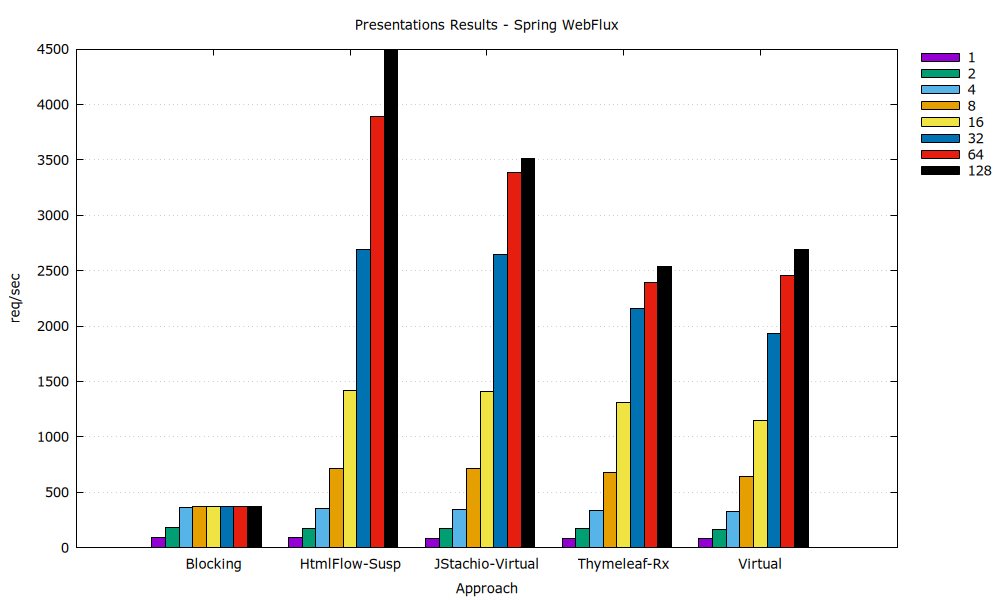
\includegraphics[width=0.8\textwidth]{./Graphs/presentations-webflux-jmeter.png}
     \caption{Throughput (requests per second) scalability results for Spring Webflux with \texttt{Presentations} class}\label{fig:presentations-webflux-jmeter}
\end{figure}

The results in Figure~\ref{fig:presentations-webflux-jmeter} show that when
using blocking template engines with a separate coroutine dispatcher, the
engines are unable to scale effectively beyond 4 concurrent users. In contrast,
\textit{HtmlFlow-Susp} scales up to 128 concurrent users, achieving 4,487
requests per second. When blocking approaches are executed in the context of
Virtual Threads—thus enabling non-blocking I/O—the engines scale up to 64
concurrent users, with Jstachio using Virtual Threads reaching 3,514 requests
per second. The Thymeleaf implementation using the reactive View Resolver
driver scales up to 32 concurrent users, achieving a lower maximum throughput
of 2,559 requests per second.

It is important to note that the differences in scalability and throughput
between the \textit{HtmlFlow-Susp}, \textit{Jstachio-Virtual}, and
\textit{Thymeleaf-Rx} approaches may be influenced by the specific template
engines used, rather than the approach itself. When comparing the
\textit{Reactive}, \textit{Suspendable}, and \textit{Virtual} approaches
specifically with HtmlFlow, we found that all three achieve similar
performance: HtmlFlow using a blocking approach with Virtual Threads reaches
4,691 requests per second, while HtmlFlow using a reactive approach achieves
4,792 requests per second.

\begin{figure}[h]
     \centering
     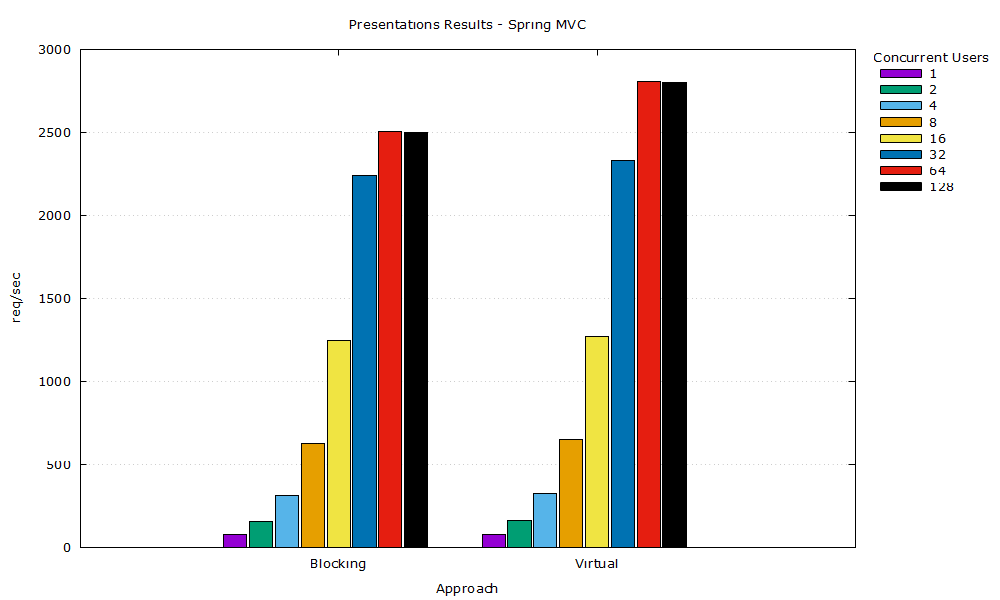
\includegraphics[width=0.8\textwidth]{./Graphs/presentations-springmvc-jmeter.png}
     \caption{Throughput (requests per second) scalability results for Spring MVC with \texttt{Presentations} class}\label{fig:presentations-springmvc-jmeter}
\end{figure}

% The results for the Spring MVC implementation, shown in
% Figure~\ref{fig:presentations-springmvc-jmeter}, compare two approaches:
% \textit{Blocking}, which uses platform threads with \texttt{StreamingResponseBody},
% and \textit{Virtual}, which uses Virtual Threads. Both approaches scale
% effectively up to 128 concurrent users, with the Virtual Thread approach
% achieving a slightly higher throughput of 9,000 requests per second. However,
% these values are slightly lower than those observed in the Spring WebFlux
% implementation.
The results for the Spring MVC implementation, shown in
Figure~\ref{fig:presentations-springmvc-jmeter}, compare two synchronous
approaches: \textit{Blocking}, which uses platform threads with
\texttt{StreamingResponseBody}, and \textit{Virtual}, which uses Virtual
Threads. Since Spring MVC follows a thread-per-request architecture, the
asynchronous approaches—\textbf{Reactive} and \textbf{Suspendable}—described in
Section~\ref{sec:bench} are not applicable. Both the \textit{Blocking} and
\textit{Virtual} strategies scale effectively up to 32 concurrent users, with
the Virtual Threads approach achieving a slightly higher maximum throughput of
2,797 requests per second, compared to 2,498 requests per second for the
blocking approach. These results indicate that while Spring MVC can handle a
moderate level of concurrency, it does not reach the scalability of the
reactive or suspendable approaches available in Spring WebFlux. Furthermore,
Spring MVC does not enable Progressive Server-Side Rendering (PSSR) for the
tested templates, as previously discussed in Section~\ref{sec:bench}.

\begin{figure}[h]
     \centering
     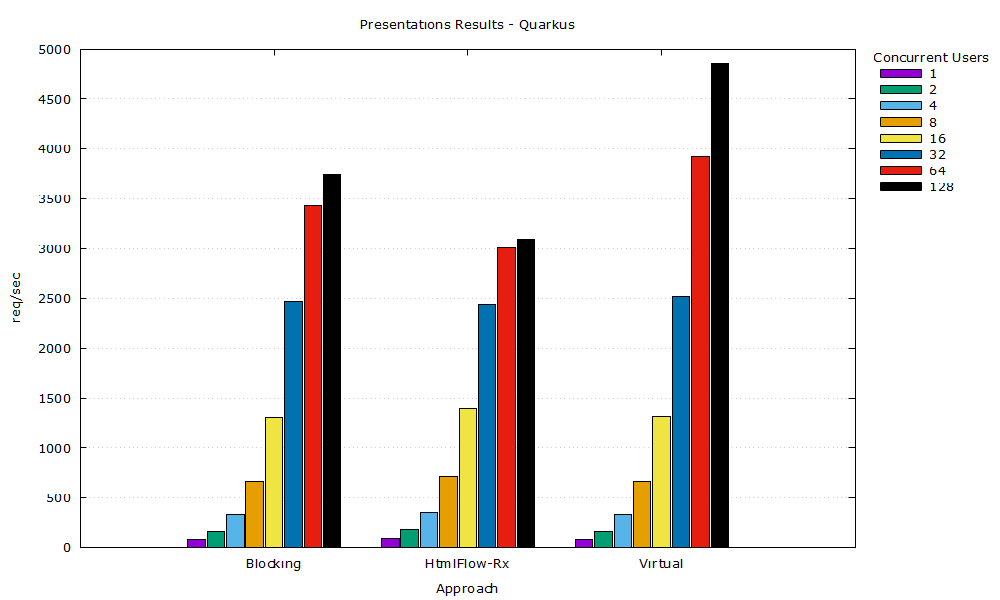
\includegraphics[width=0.8\textwidth]{./Graphs/presentations-quarkus-jmeter.png}
     \caption{Throughput (requests per second) scalability results for Quarkus with \texttt{Presentations} class}\label{fig:presentations-quarkus-jmeter}
\end{figure}

The results for the Quarkus implementation, shown in
Figure~\ref{fig:presentations-quarkus-jmeter}, indicate that Quarkus handles
synchronous approaches more efficiently than Spring WebFlux. The blocking
engines scale up to 64 concurrent users, achieving up to 3,744 requests per
second. When using Virtual Threads, the throughput increases even further,
reaching 4,856 requests per second, allowing scalability up to 128 users. This
demonstrates that Quarkus's implementation of Virtual Threads is effective for
enabling PSSR\@, and comparable to the \textit{Suspendable} and
\textit{Reactive} approaches used in Spring WebFlux in terms of scalability and
throughput.

Additionally, \textit{HtmlFlow-Rx}, a reactive implementation of the HtmlFlow
template engine (equivalent to the approach shown in
Listing~\ref{lst:presentation-observable}) that utilizes Quarkus's reactive
programming model, achieved a lower throughput than the the \textit{Blocking}
and \textit{Virtual} approaches—3,088 requests per second. This demonstrates
that Quarkus's reactive programming model is effective for enabling PSSR\@,
although it does not achieve the same level of performance or scalability as
the same approach in Spring WebFlux, stagnating after 32 concurrent users.

\subsection{Scalability results for the \texttt{Stocks} class} \label{sec:stocks-results}

\begin{figure}[h]
     \centering
     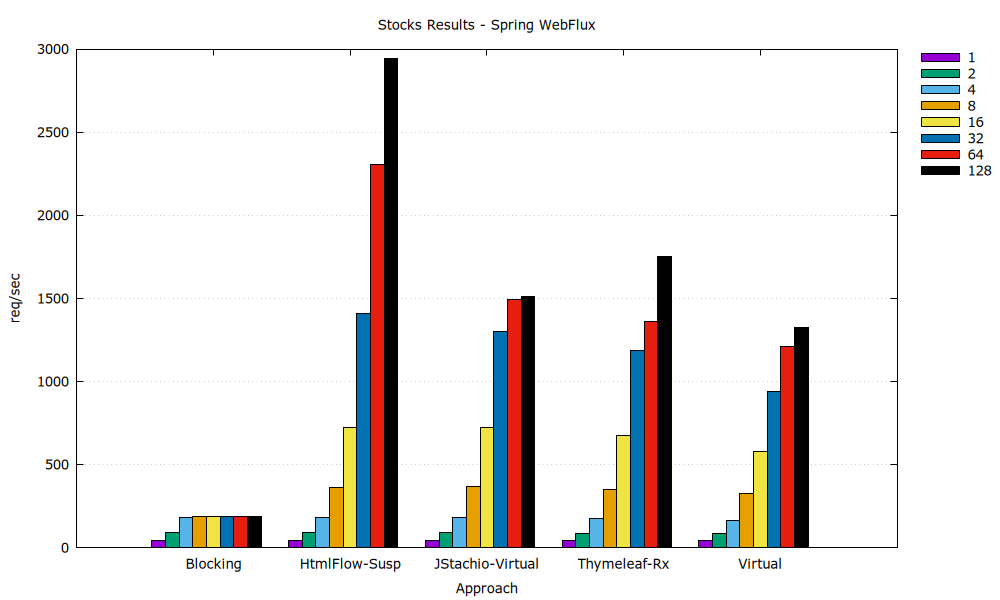
\includegraphics[width=0.8\textwidth]{./Graphs/stocks-webflux-jmeter.png}
     \caption{Throughput (requests per second) scalability results for Spring Webflux with \texttt{Stocks} class}\label{fig:stocks-webflux-jmeter}
\end{figure}

The results in Figure~\ref{fig:stocks-webflux-jmeter} use the same template
engines and approaches as the previous benchmark, but with a more complex data
model: the Stock class, which includes 20 instances and approximately two times
as many data bindings. With this data model, the scalability of the engines
remains largely unchanged; however, throughput is reduced across all engines.
Compared to the Presentation benchmark, Jstachio using virtual threads
experienced a more pronounced decrease in performance relative to the
\textit{Reactive} and \textit{Suspending} approaches, with Jstachio using
Virtual Threads now achieving 1,509 requests per second, compared to 1,750
requests per second achieved by the Thymeleaf implementation using the reactive
View Resolver driver.

It is again important to note that the differences in scalability and
throughput between the \textit{HtmlFlow-Susp}, \textit{Jstachio-Virtual}, and
\textit{Thymeleaf-Rx} approaches may be influenced by the specific template
engines used, rather than the approach itself. When comparing the
\textit{Reactive}, \textit{Suspendable}, and \textit{Virtual} approaches
specifically with HtmlFlow, we found that all three achieve similar
performance: HtmlFlow using a blocking approach with Virtual Threads reaches
3,090 requests per second, while HtmlFlow using a reactive approach achieves
3,026 requests per second. This indicates that the more pronounced decrease in
performance for Jstachio using Virtual Threads is likely due to the specific
implementation of the template engine, rather than the use of Virtual Threads
itself.

The overall throughput reduction across all engines is expected, as the Stock
class contains more data properties than the \texttt{Presentation} class,
adding overhead related to the data binding process of each template engine.

\begin{figure}[h]
     \centering
     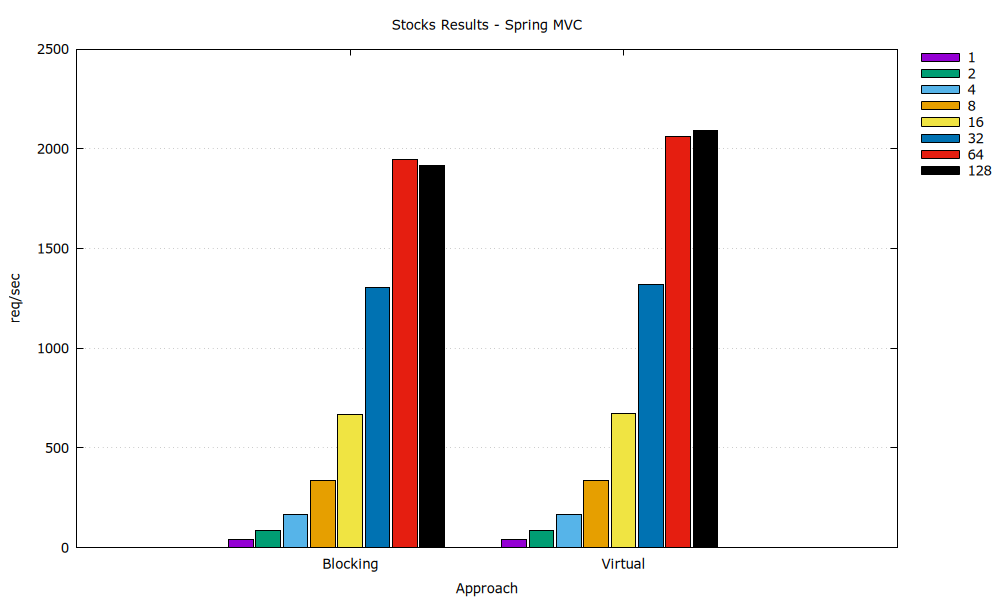
\includegraphics[width=0.8\textwidth]{./Graphs/stocks-springmvc-jmeter.png}
     \caption{Throughput (requests per second) scalability results for Spring MVC with \texttt{Stocks} class}\label{fig:stocks-springmvc-jmeter}
\end{figure}

The results shown in Figure~\ref{fig:stocks-springmvc-jmeter} indicate that the
Spring MVC implementation using the blocking approach with
\texttt{StreamingResponseBody} achieves a throughput of up to 1,916 requests
per second, with no significant improvement observed when using Virtual
Threads. Both approaches scale effectively up to 64 concurrent users. Although
these approaches achieve higher throughput in Spring MVC than in Spring
WebFlux, their overall performance remains lower than that of the reactive and
suspendable approaches.

\begin{figure}[h]
     \centering
     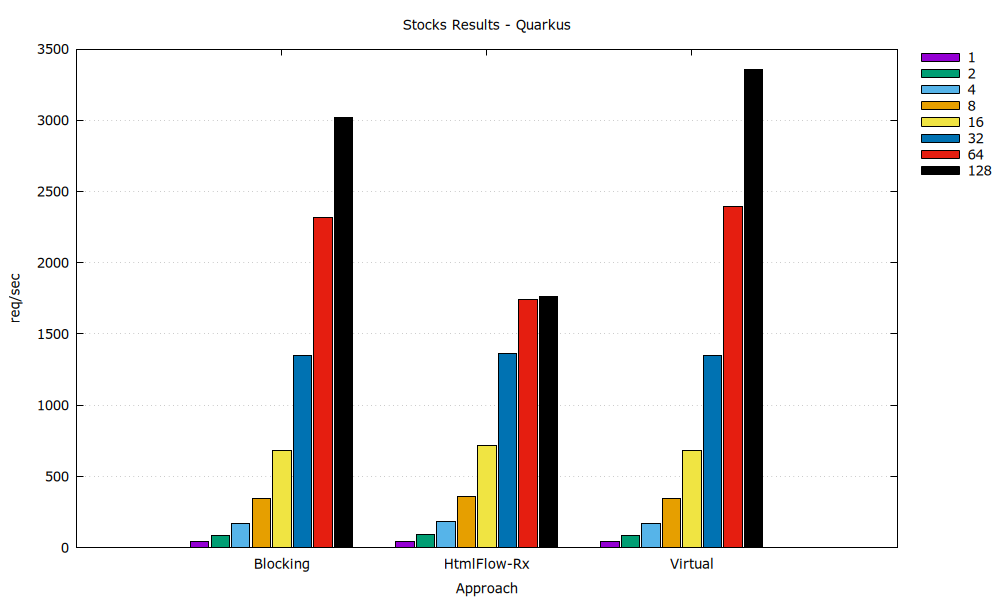
\includegraphics[width=0.8\textwidth]{./Graphs/stocks-quarkus-jmeter.png}
     \caption{Throughput (requests per second) scalability results for Quarkus with \texttt{Stocks} class}\label{fig:stocks-quarkus-jmeter}
\end{figure}

The results depicted in Figure~\ref{fig:stocks-quarkus-jmeter} show that the
Quarkus synchronous approaches scale effectively up to 128 concurrent users,
achieving performance comparable to the Spring WebFlux implementation. The
blocking approach reaches a throughput of 3,019 requests per second, while the
Virtual Threads approach achieves a throughput of 3,357 requests per second. In
addition to the synchronous engines, the \textit{HtmlFlow-Rx} approach also
achieves a throughput of 1760 requests per second, indicating that this
approach achieves lower performance in Quarkus than in Spring WebFlux, where it
reached 3,026 requests per second, as previously mentioned.

The results of the benchmarks show that non-blocking engines—whether using
reactive programming, Kotlin coroutines, or Java Virtual Threads—are able to
scale effectively, supporting between 32 and 128 concurrent users depending on
the approach and framework. Out of all the tested frameworks, Spring Webflux
showed itself the most effective at enabling PSSR, mostly due to its native
support for publish-subscribe interfaces, allowing for content to be streamed
as data becomes available, instead of when the response buffer is flushed.
Quarkus also enabled PSSR effectively, but it required additional configuration
of the \texttt{OutputBuffer} size to achieve the same results as Spring
Webflux. The Spring MVC implementation, on the other hand, did not enable PSSR
for the tested templates.

However, it is important to acknowledge the limitations of our chosen data
models for generalizability. The tested templates used relatively simple data
structures with limited nesting and straightforward property bindings.
Real-world applications often involve deeply nested data structures, complex
conditional logic, and iterative rendering over thousands of items. Under such
conditions, we anticipate significantly different performance characteristics:
increased memory consumption due to object traversal overhead, higher CPU
utilization for complex evaluations, and altered scalability patterns where
non-blocking approaches may become more advantageous. The performance
degradation observed with our Stock class benchmark—which merely doubled the
number of properties—suggests that higher template complexity would result in
substantially higher performance degradation. Future work should investigate
these scenarios with more realistic data models to better understand
performance boundaries and optimization strategies for complex PSSR
implementations.

\subsection{Memory Consumption and Resource Utilization Analysis}
\label{sec:memory-analysis}

This section evaluates the memory and CPU resource usage characteristics of
structured concurrency approaches, specifically comparing Virtual Threads and
suspendable coroutines.

Resource utilization data was collected using VisualVM during 30-second
benchmark runs, capturing detailed CPU and memory usage patterns under
sustained load conditions. Each profiling session monitored system performance
during the 1 to 128 concurrent user load test, providing comprehensive insights
into runtime behavior.

\subsubsection{Virtual Threads vs Structured Concurrency}

\begin{center}
     \begin{minipage}[t]{0.48\textwidth}
          \centering
          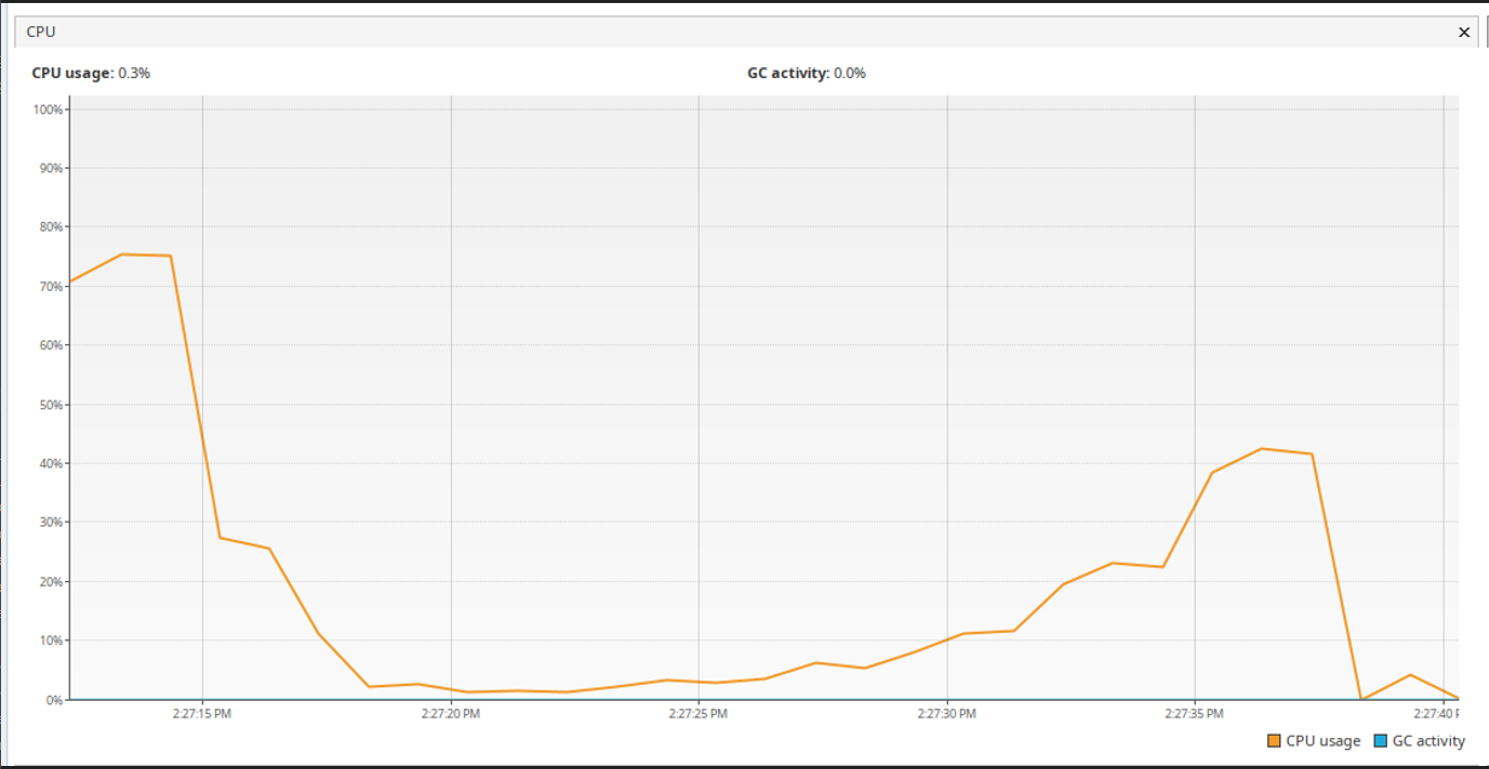
\includegraphics[width=1.0\textwidth,height=1.0\textwidth]{./Graphs/cpu-susp.png}
          \captionof{figure}{CPU utilization profiling with HtmlFlow-Susp in Spring WebFlux during 30-second load test}
          \label{fig:cpu-susp}
     \end{minipage}
     \hfill
     \begin{minipage}[t]{0.48\textwidth}
          \centering
          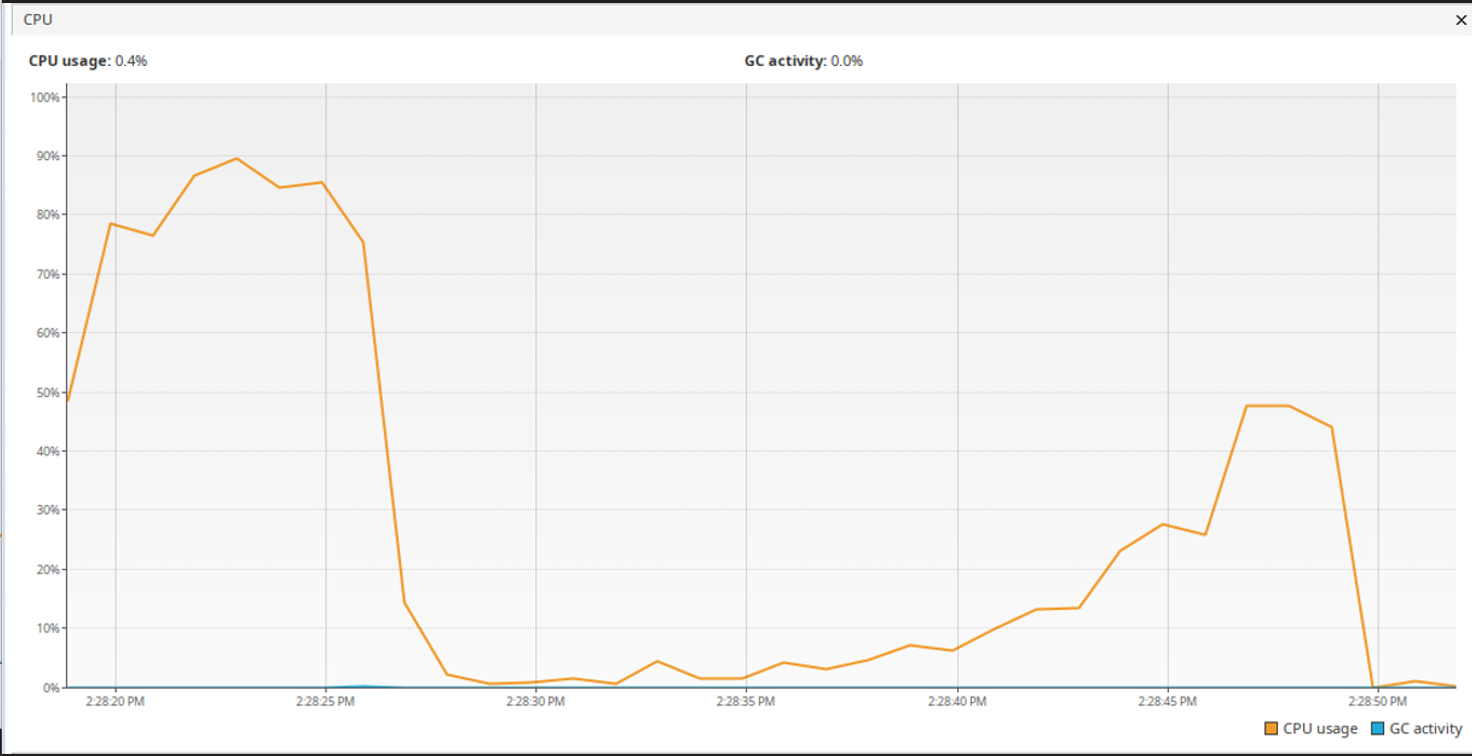
\includegraphics[width=1.0\textwidth,height=1.0\textwidth]{./Graphs/cpu-virt.png}
          \captionof{figure}{CPU utilization profiling with HtmlFlow-Virtual in Spring WebFlux during 30-second load test}
          \label{fig:cpu-virt}
     \end{minipage}
\end{center}

\begin{center}
     \begin{minipage}[t]{0.48\textwidth}
          \centering
          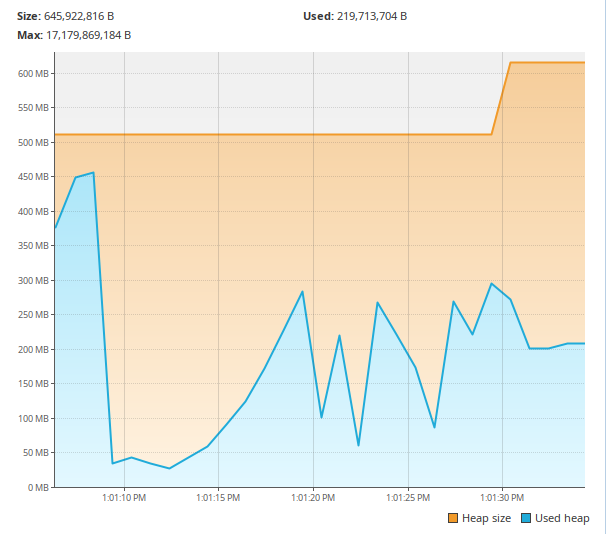
\includegraphics[width=1.0\textwidth,height=1.0\textwidth]{./Graphs/mem-susp.png}
          \captionof{figure}{Memory utilization and garbage collection behavior with HtmlFlow-Susp in Spring WebFlux during 30-second load test}
          \label{fig:gc-susp}
     \end{minipage}
     \hfill
     \begin{minipage}[t]{0.48\textwidth}
          \centering
          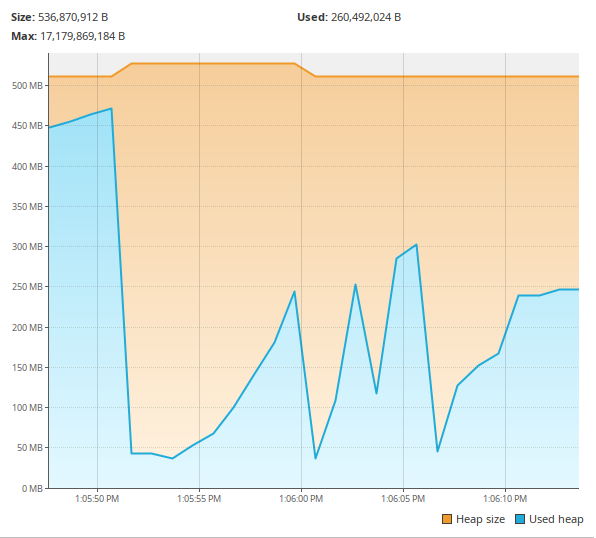
\includegraphics[width=1.0\textwidth,height=1.0\textwidth]{./Graphs/mem-virt.png}
          \captionof{figure}{Memory utilization and garbage collection behavior with HtmlFlow-Virtual in Spring WebFlux during 30-second load test}
          \label{fig:gc-virt}
     \end{minipage}
\end{center}

Figures~\ref{fig:cpu-virt} and~\ref{fig:cpu-susp} show CPU utilization profiles
for the \texttt{HtmlFlow-Virtual} and \texttt{HtmlFlow-Susp} implementations,
respectively. The subsequent gradual increase in CPU utilization reflects the
ramp-up of concurrent users during the benchmark. \texttt{HtmlFlow-Virtual}
exhibits a distinctive bell-shaped curve, rapidly climbing from near-zero to
peak CPU usage of around 50\% during the sustained load phase, maintaining
moderate utilization during the test period, and then dropping sharply back to
baseline. \texttt{HtmlFlow-Susp} displays a similar pattern but with a slightly
lower peak CPU utilization of approximately 42\%, showing marginally lower
intensive CPU usage during the sustained load phase. Both profiles demonstrate
comparable resource consumption patterns, with the virtual thread
implementation showing only slightly higher CPU demands. The GC activity
indicators in both profiles remain relatively low throughout the test duration,
confirming that garbage collection overhead does not significantly impact CPU
utilization in either approach.

Figures~\ref{fig:gc-susp} and~\ref{fig:gc-virt} show similar memory usage for
both approaches, with peaks around 300~MB during load. The initial spike to
450~MB in both graphs corresponds to the applications' bootstrapping phase.
Overall, these results indicate that under the tested conditions, Virtual
Threads and suspendable coroutines exhibit comparable memory consumption.

Virtual Threads allocate a full call stack per thread, which is unmounted and
stored on the heap when suspended (e.g., during blocking I/O). In contrast,
Kotlin coroutines compile into state machines that capture only the minimal
execution state needed to resume computation. This typically allows coroutines
to scale more efficiently in terms of memory usage, especially under high
concurrency.

\section{Discussion}

Beronić et al.~\cite{9803765} compared different structured concurrency
constructs in Java and Kotlin in the context of a multithreaded HTTP server.
Their benchmark scenario differs from ours: their server awaited incoming
requests and, upon receiving one, executed a task involving object creation,
writing the object's information to a file, and returning the data as a
response. Consistent with our findings, they concluded that both Kotlin's
coroutines and Java's virtual threads offer significant performance
improvements over traditional JVM-based threads in concurrent applications.

Our results diverge from theirs regarding memory usage. They reported lower
heap usage for Java virtual threads (16–64~MB) compared to Kotlin coroutines
(52–99~MB), which contrasts with our measurements. This discrepancy may be
attributed to the different workloads: while their benchmark includes a single
I/O read-write operation per request, our experiments focus exclusively on
read-only I/O tasks.

The work of Navarro et al.~\cite{navarro2023considerations} focused on the
performance of Quarkus, which relies on Eclipse Vert.x~\cite{vertx}, itself
built on top of Netty~\cite{netty}. This represents a similar environment to
the one evaluated in our experiments with Quarkus. Their study also emphasized
template rendering, using a blocking HTML template engine (Qute). The benchmark
they employed is the Fortunes
test\footnote{\url{https://www.techempower.com/benchmarks}}, which involves
rendering a simple HTML table with only two data bindings per row.

Their results show that Quarkus with Virtual Threads outperformed the
traditional thread-per-request model under increased concurrency. Moreover,
compared to the reactive model, virtual threads demonstrated competitive
performance, particularly when executing blocking operations within template
engines. In contrast, our experiments revealed that the reactive approach
underperforms relative to virtual threads, likely due to the significantly
larger number of data bindings in our use cases—namely, the
\texttt{Presentation} and \texttt{Stock} models.

The work of Šimatović et al.\cite{vsimatovic2025evaluating} presents an
evaluation of Java Virtual Threads under different garbage collectors. They
explored three types of workloads, only one of which was based on a web
application scenario. This scenario replicated large-scale web scraping by
executing 1,000 parallel tasks, each consisting of an I/O-bound operation
followed by CPU-bound string processing.

In this workload, garbage collection activity remained low across all
collectors, indicating reduced memory pressure. These findings suggest that
Virtual Threads improve memory allocation efficiency and reduce the frequency
of garbage collection cycles—particularly when used with concurrent garbage
collectors.

Our observations suggest that the choice between Virtual Threads and
suspendable coroutines should be guided by both runtime behavior and
development constraints. Virtual Threads offer the compelling advantage of
preserving synchronous programming semantics while achieving competitive
performance across moderate to high-load scenarios—a significant benefit for
teams migrating existing codebases or working with legacy template engines.
Suspendable coroutines, while requiring developers to adopt asynchronous
programming paradigms, may provide greater efficiency in scenarios involving
high concurrency, deeper call stacks, or highly dynamic workloads.

The framework-specific variations observed in our results—particularly the
performance differences between Spring WebFlux and Quarkus
implementations—suggest that the underlying reactive runtime architecture
significantly influences the effectiveness of each approach. This finding
underscores the importance of considering not only the concurrency model but
also the specific framework ecosystem when making architectural decisions for
PSSR implementations.

\chapter{Conclusion}

In recent decades, non-blocking I/O has become the standard approach for building
highly responsive and scalable web servers. However, traditional synchronous
programming models are not compatible with non-blocking APIs, which typically
rely on callback-based conventions such as
\textit{continuation-passing style} (CPS)~\cite{scheme} or
\textit{promises}~\cite{promise}. These approaches not only hinder
sequential readability but also increase code verbosity, making them more
error-prone.
Alternatives like the \texttt{async}/\texttt{await} idiom~\cite{async_await}
or \textit{suspend functions}~\cite{elizarov2021coroutines} simplify
asynchronous programming by mimicking a sequential style without blocking
threads.
Recent proposals~\cite{carvalho2023async,wise2024pssr} have applied contemporary
asynchronous idioms to SSR web templates, demonstrating how they can overcome
the scalability bottlenecks present in traditional web template engines.

As an alternative, Java Virtual Threads can be applied to any blocking I/O call,
leveraging the Java runtime to transparently intercept and convert it into non-blocking I/O,
without requiring any changes to the calling code or exposing its internal complexities.
In this work, we explored how this technique can be applied to traditional
web template engines and whether it can achieve performance competitive with
reactive approaches provided by frameworks such as Thymeleaf~\cite{webflux} and HtmlFlow~\cite{htmlflow}.
Our benchmarks across Spring WebFlux, Spring MVC, and Quarkus show that synchronous
non-blocking execution using virtual threads consistently delivers performance
comparable to asynchronous non-blocking approaches under high concurrency.
These findings highlight virtual threads as a promising alternative to complex
asynchronous programming models, offering a simpler development experience
without compromising scalability or responsiveness.

% 
% All figures and tables should be cited in the main text as Figure~\ref{fig1},
% Table~\ref{tab1}, etc.
% 
% \begin{figure}[H]
% 	%\isPreprints{\centering}{} % Only used for preprints
% 	\includegraphics[width=4 cm]{Definitions/logo-mdpi}
% 	\caption{This is a figure. Schemes follow the same formatting.\label{fig1}}
% \end{figure}
% \unskip
% 
% % Example of a figure that spans the whole page width and with subfigures. The same concept works for tables, too.
% \begin{figure}[H]
% 	%\isPreprints{}{% This command is only used for ``preprints''.
% 	\begin{adjustwidth}{-\extralength}{0cm}
% 		\centering
% 		%} % If the paper is ``preprints'', please uncomment this parenthesis.
% 		\subfloat[\centering]{\includegraphics[width=7.0cm]{Definitions/logo-mdpi}}
% 		%\hfill
% 		\subfloat[\centering]{\includegraphics[width=7.0cm]{Definitions/logo-mdpi}}\\
% 		\subfloat[\centering]{\includegraphics[width=7.0cm]{Definitions/logo-mdpi}}
% 		%\hfill
% 		\subfloat[\centering]{\includegraphics[width=7.0cm]{Definitions/logo-mdpi}}
% 		%\isPreprints{}{% This command is only used for ``preprints''.
% 	\end{adjustwidth}
% 	%} % If the paper is ``preprints'', please uncomment this parenthesis.
% 	\caption{This is a wide figure. Schemes follow the same formatting. If there are multiple panels, they should be listed as: (\textbf{a}) Description of what is contained in the first panel. (\textbf{b}) Description of what is contained in the second panel. (\textbf{c}) Description of what is contained in the third panel. (\textbf{d}) Description of what is contained in the fourth panel. Figures should be placed in the main text near to the first time they are cited. A caption on a single line should be centered.\label{fig2}}
% \end{figure}
% 
% \begin{table}[H]
% 	\caption{This is a wide table.\label{tab2}}
% 	%\isPreprints{\centering}{% This command is only used for ``preprints''.
% 	\begin{adjustwidth}{-\extralength}{0cm}
% 		%} % If the paper is ``preprints'', please uncomment this parenthesis.
% 		%\isPreprints{\begin{tabularx}{\textwidth}{CCCC}}{% This command is only used for ``preprints''.
% 		\begin{tabularx}{\fulllength}{CCCC}
% 			%} % If the paper is ``preprints'', please uncomment this parenthesis.
% 			\toprule
% 			\textbf{Title 1}              & \textbf{Title 2} & \textbf{Title 3} & \textbf{Title 4} \\
% 			\midrule
% 			\multirow[m]{3}{*}{Entry 1 *} & Data             & Data             & Data             \\
% 			                              & Data             & Data             & Data             \\
% 			                              & Data             & Data             & Data             \\
% 			\midrule
% 			\multirow[m]{3}{*}{Entry 2}   & Data             & Data             & Data             \\
% 			                              & Data             & Data             & Data             \\
% 			                              & Data             & Data             & Data             \\
% 			\bottomrule
% 		\end{tabularx}
% 		%		\isPreprints{}{% This command is only used for ``preprints''.
% 	\end{adjustwidth}
% 	%} % If the paper is ``preprints'', please uncomment this parenthesis.
% 	\noindent{\footnotesize{* Tables may have a footer.}}
% \end{table}
% 
%\begin{listing}[H]
%\caption{Title of the listing}
%\rule{\columnwidth}{1pt}
%\raggedright Text of the listing. In font size footnotesize, small, or normalsize. Preferred format: left aligned and single spaced. Preferred border format: top border line and bottom border line.
%\rule{\columnwidth}{1pt}
%\end{listing}

%%%%%%%%%%%%%%%%%%%%%%%%%%%%%%%%%%%%%%%%%%
% \section{Conclusions}
% 
% This section is not mandatory, but can be added to the manuscript if the
% discussion is unusually long or complex.

%%%%%%%%%%%%%%%%%%%%%%%%%%%%%%%%%%%%%%%%%%
\vspace{6pt}

%%%%%%%%%%%%%%%%%%%%%%%%%%%%%%%%%%%%%%%%%%
%% optional
%\supplementary{The following supporting information can be downloaded at:  \linksupplementary{s1}, Figure S1: title; Table S1: title; Video S1: title.}

% Only for journal Methods and Protocols:
% If you wish to submit a video article, please do so with any other supplementary material.
% \supplementary{The following supporting information can be downloaded at: \linksupplementary{s1}, Figure S1: title; Table S1: title; Video S1: title. A supporting video article is available at doi: link.}

% Only used for preprtints:
% \supplementary{The following supporting information can be downloaded at the website of this paper posted on \href{https://www.preprints.org/}{Preprints.org}.}

% Only for journal Hardware:
% If you wish to submit a video article, please do so with any other supplementary material.
% \supplementary{The following supporting information can be downloaded at: \linksupplementary{s1}, Figure S1: title; Table S1: title; Video S1: title.\vspace{6pt}\\
%\begin{tabularx}{\textwidth}{lll}
%\toprule
%\textbf{Name} & \textbf{Type} & \textbf{Description} \\
%\midrule
%S1 & Python script (.py) & Script of python source code used in XX \\
%S2 & Text (.txt) & Script of modelling code used to make Figure X \\
%S3 & Text (.txt) & Raw data from experiment X \\
%S4 & Video (.mp4) & Video demonstrating the hardware in use \\
%... & ... & ... \\
%\bottomrule
%\end{tabularx}
%}

%%%%%%%%%%%%%%%%%%%%%%%%%%%%%%%%%%%%%%%%%%
\authorcontributions{Conceptualization, B.P. and F.M.C; methodology, B.P and F.M.C; software, B.P and F.M.C; validation, B.P and F.M.C; formal analysis, B.P and F.M.C; investigation, B.P and F.M.C; resources, B.P and F.M.C; data curation, B.P and F.M.C; writing---original draft preparation,B.P and F.M.C; writing---review and editing, B.P and F.M.C; supervision, F.M.C.; project administration, F.M.C. All authors have read and agreed to the published version of the manuscript.}

\funding{This research received no external funding}

\institutionalreview{This study did not involve human subjects or personal data; therefore, Institutional Review Board approval was not required.}

\dataavailability{The data presented in this study are available in Github at \url{https://github.com/xmlet/comparing-non-blocking-progressive-ssr}.}

% Only for journal Drones
%\durcstatement{Current research is limited to the [please insert a specific academic field, e.g., XXX], which is beneficial [share benefits and/or primary use] and does not pose a threat to public health or national security. Authors acknowledge the dual-use potential of the research involving xxx and confirm that all necessary precautions have been taken to prevent potential misuse. As an ethical responsibility, authors strictly adhere to relevant national and international laws about DURC. Authors advocate for responsible deployment, ethical considerations, regulatory compliance, and transparent reporting to mitigate misuse risks and foster beneficial outcomes.}

% Only for journal Nursing Reports
%\publicinvolvement{Please describe how the public (patients, consumers, carers) were involved in the research. Consider reporting against the GRIPP2 (Guidance for Reporting Involvement of Patients and the Public) checklist. If the public were not involved in any aspect of the research add: ``No public involvement in any aspect of this research''.}
%
%% Only for journal Nursing Reports
%\guidelinesstandards{Please add a statement indicating which reporting guideline was used when drafting the report. For example, ``This manuscript was drafted against the XXX (the full name of reporting guidelines and citation) for XXX (type of research) research''. A complete list of reporting guidelines can be accessed via the equator network: \url{https://www.equator-network.org/}.}
%
%% Only for journal Nursing Reports
%\useofartificialintelligence{Please describe in detail any and all uses of artificial intelligence (AI) or AI-assisted tools used in the preparation of the manuscript. This may include, but is not limited to, language translation, language editing and grammar, or generating text. Alternatively, please state that “AI or AI-assisted tools were not used in drafting any aspect of this manuscript”.}

\conflictsofinterest{The authors declare no conflicts of interest.}

%%%%%%%%%%%%%%%%%%%%%%%%%%%%%%%%%%%%%%%%%%
%\isPreprints{} % If the paper is ``preprints'', please uncomment this parenthesis.
	%\printendnotes[custom] % Un-comment to print a list of endnotes

	\reftitle{References}

	% Please provide either the correct journal abbreviation (e.g. according to the “List of Title Word Abbreviations” http://www.issn.org/services/online-services/access-to-the-ltwa/) or the full name of the journal.
	% Citations and References in Supplementary files are permitted provided that they also appear in the reference list here. 

	%=====================================
	% References, variant A: external bibliography
	%=====================================
	\bibliography{bibliography.bib}

	%=====================================
	% References, variant B: internal bibliography
	%=====================================

	\PublishersNote{}
	%\isPreprints{} % If the paper is ``preprints'', please uncomment this parenthesis.
\end{document}

